\chapter{Extension of the Rule-Based Lloyd Algorithm to 3D\label{chap:rbl}}
\section{Introduction}
    \subsection{Motivation}
        Motivation in using \ac{RBL} algorithm offers communication-less approach for guiding multiple agents from point A to point B.
        It relies on global positioning data together with onboard sensors that provide information about the surrounding environment.
        So far, the algorithm has mainly been tested in 2D scenarios with a fixed altitude, and the results have looked promising. 
        This were the main motivation factors to try and extend it to full 3D navigation, where altitude and sensor orientation also play a role.

    \subsection{Problem Statement}
        The primary challenge that was addressed involved the extension of an existing 2D algorithm into a 3D space. 
        To achieve improved results in this higher dimension, new rules controling vertical exploration were introduced. 
        The subsequent sections of this chapter detail the fundamental principles of the \ac{RBL} algorithm, with specific attention devoted to its application in both 2D and 3D environments. 
        The distinct rules governing the algorithm's behavior in these two dimensions are described separately to provide clarity. 
        Finally, the chapter concludes in the presentation and evaluation of simulation experiments designed to assess the efficiency of the proposed 3D extension and the impact of the introduced vertical exploration rules.

    \subsection{Objectives}
        \begin{itemize}
            \item   Enhance the convergence speed of agents towards their goals by promoting exploration, with  focus on the vertical exploration.
            \item   Demonstrate the algorithm's enhanced applicability, achieved by extending goal placement to the z-axis.
        \end{itemize}

    \subsection{Chapter Overview}
        The principles of the \ac{RBL} algorithm, presented in \cite{rbl_paper}, form the basis of the work in this chapter. 
        These principles are clarified and modified to address the challenges of 3D extension.  
        The chapter details the fundamental principles of RBL in 2D and 3D spaces, describes the specific rules applied to enhance convergence, and concludes with a series of simulation scenarios designed to demonstrate the performance of the proposed solution.

\section{Basic principles of Rule-Based Lloyd Algorithm}

    \subsection{Overview}        
        The algorithm is a communication-less approach designed to navigate agents from point A to point B. 
        It relies on global positioning data, such as GPS or alternative methods for obtaining global coordinates, combined with sensor inputs that provide information about the agent's environment. 
        These sensors can include LiDAR, depth cameras, or standard cameras with estimation techniques, allowing the agent to detect and avoid obstacles or other agents. 
        The algorithm enables autonomous navigation without requiring direct communication between agents, making it suitable for scalable and decentralized applications.

    \subsection{Applications and Limitations in 2D}
        Modern robotics relies on the capability to navigate from point A to point B.
        Navigation plays a crucial role in various robotic applications, such as \ac{UGV}s, which are commonly used in manufacturing and logistics. 
        \ac{UGV}s typically follow predefined 2D trajectories guided by visual \cite{vision_navigation}, magnetic \cite{magnetic_navigation}, or LiDAR-based navigation \cite{lidar_navigation}. 
        Additionally, 2D navigation is widely employed in robotic vacuum cleaners, enabling them to systematically cover an area while avoiding obstacles.

        An obvious limitation for algorithms in 2D is scalability. 
        As the number of agents in a system increases, the complexity of managing their movements and coordination also grows significantly.
        Obstacle avoidance in 2D can also be less efficient compared to 3D environments, as agents have fewer options for evading obstacles. 
        In 3D, agents can change their altitude in addition to their horizontal trajectory, giving them more freedom to maneuver around obstacles.

    \subsection{Key principles}
        RBL ensures convergence to the goal and provides sufficient conditions for achieving it. 
        The problem involves individual control of $N$ agents from their initial position $\mathbf{p}_i(0)$ toward a goal region, represented as circle.
        This goal region is denoted as $G(\mathbf{g}_i, r_g)$, where $\mathbf{g}_i$ is center and $r_g$ is radius of goal region. 
        The agent is progressing towards its designated destination, $\mathbf{d}_i$.
        Each agent is knows of its current position $\mathbf{p}_i$, encumbrance $\delta_i$, which determines safe space around agent.
        Additionally, each agent also knows the positions and encumbrances of its neighboring agents $\mathbf{\mathcal{N}_i}$, agent $j \in \mathbf{\mathcal{N}_i}$ if $||\mathbf{p}_i - \mathbf{p}_j|| \leq 2r_{s,i}$, where $r_{s,i}$ is denoted as half of the sensing radius of the i-th agent.
        For simplicity $r_{s,i}$ is considered to be same for all agents, therefore $r_{s,i} = r_s$. 

        The core objective of the algorithm is to minimize the coverage cost function, which accounts for the distribution of agents and obstacles over the environment. 
        This function is expressed as:
        \begin{equation}
            J_{cov}(\mathbf{p}) = \sum_{i=1}^{N} \int_{\mathcal{V}_i} \lVert\mathbf{q}-\mathbf{p}_i\rVert^2 \varphi_i (\mathbf{q})d\mathbf{q},
            \label{coverage_cost_function}
        \end{equation}
        where $\mathbf{p}_i$ is the position of agent $i$, $\mathcal{V}_i$ is the Voronoi cell of the i-th robot, $\lVert\mathbf{q}-\mathbf{p_i}\rVert^2$ is squared Euclidian distance between point in the mission space $\mathbf{q} \in \mathcal{Q}$ and agent's position $p_i$, 
        and $\varphi_i (\mathbf{q})$ is the weighting function.

        Voronoi cell is defined as: 
        \begin{equation}
            \mathcal{V}_i = \{q \in \mathcal{Q} \lvert \lVert \mathbf{q} - \mathbf{p}_i \rVert \leq \lVert q - \mathbf{p}_j \rVert, \forall j \neq i\}
        \end{equation}
        For visual representation see \reffig{fig:voronoi_2d}. 

        However, this standard definition of Voronoi cells does not take into account the physical space occupied by the agents, or their encumbrances. 
        To address this, a Modified Voronoi cell is introduced, which takes into account the encumbrances of agents.
        This modified version adjusts the boundaries of each Voronoi cell to account for the encumbrances of neighboring agents.
        Also to enhance the algorithm performance, the Voronoi cell are scaled using a scaling parameter $\eta \in [0, 1]$.
        The modified Voronoi cell definition is as follows:
        \begin{equation}
            \label{eq:voronoi_cell_account_encum}
            \tilde{V}_i = 
            \begin{cases}
            \{ \mathbf{q} \in Q \mid \| \mathbf{q} - \mathbf{p}_i \| \leq \eta \| \mathbf{q} - \mathbf{p}_j \| \}, & \text{if } \Delta_{ij} \leq \frac{\| \mathbf{p}_i - \mathbf{p}_j \|}{2} \\
            \{ \mathbf{q} \in Q \mid \| \mathbf{q} - \mathbf{p}_i \| \leq \eta \| \mathbf{q} - \tilde{\mathbf{p}}_j \| \}, & \text{otherwise},
            \end{cases}
        \end{equation}
        $\forall j \in \mathcal{N}_i$, where $\Delta_{ij} = \delta_i + \delta_j$ and $\tilde{\mathbf{p}}_j = \mathbf{p}_j + 2(\Delta_{ij} - \frac{\| \mathbf{p}_i - \mathbf{p}_j \|}{2})\frac{ \mathbf{p}_i - \mathbf{p}_j }{\| \mathbf{p}_i - \mathbf{p}_j \|}$.
        Together with cell $\mathcal{S}_i$ defined as: 
        \begin{equation}
            \mathcal{S}_i = \{\mathbf{q} \in \mathcal{Q} | \| \mathbf{q} - \mathbf{p}_i \| \leq r_{s,i}\}
        \end{equation}
        the cell $\mathcal{A}_i$ is obtained as $\mathcal{A}_i = \tilde{V}_i \cap \mathcal{S}_i$.

        Convergence to goal region $G(\mathbf{g}_i, r_g )$ depends on the choice of weighting function that assigns weights to points $\mathbf{q}$ in the mission space $\mathcal{Q}$.
        The weighting function $\varphi_i(\mathbf{q})$ is defined as follows: 
        \begin{equation}
            \varphi_i(\mathbf{q}) = \exp\left(-\frac{\|\mathbf{q} - \mathbf{d}_i\|}{\beta_i}\right),
        \end{equation}
        where $\beta_i$ is the weighting factor for points $\mathbf{q}$, and $\mathbf{d}_i$ represents the current destination of the agent. 
        The destination is computed as follows:
        \begin{equation}
            \mathbf{d}_i = \mathbf{p}_i + R(\theta)(\mathbf{g}_i - \mathbf{p}_i)
        \end{equation}
        where $R$ is the azimuthal rotation.
        Rules: 
        \begin{itemize}
            \item \textbf{Weighting rule}
                \begin{equation}
                    \label{eqn:beta_weighting}
                    \dot{\beta}_i(A_i) = 
                    \begin{cases}
                        -k & \text{if } \beta_i > \beta_{min} \land \|\mathbf{c}_{A_i} - \mathbf{p}_i\| < d_1 \land \|\mathbf{c}_{A_i} - \mathbf{c}_{\mathcal{S}_i}\| > d_2  \\
                        0  & \text{if } \beta_i \leq \beta_{min} \land \|\mathbf{c}_{A_i} - \mathbf{p}_i\| < d_1 \land \|\mathbf{c}_{A_i} - \mathbf{c}_{\mathcal{S}_i}\| > d_2  \\
                        -(\beta_i - \beta_i^D) & \text{otherwise}
                    \end{cases}
                \end{equation}
                where the first case decreases $\beta_i$ over time, the second case ensures that $\beta_i$ does not decrease below its minimum threshold $\beta_{min}$ (saturation) and the third case provides a general update rule when the previous conditions are not met.
            \item \textbf{Azimuth update rule}
                \begin{equation}
                    \label{eqn:azimuth_2d}
                    \dot{\theta}_i = 
                    \begin{cases}
                        k  & \text{if } \theta < \frac{\pi}{2} \land \|\mathbf{c}_{\mathcal{A}_i} - \mathbf{c}_{\mathcal{S}_i}\| > d_4 \land \|\mathbf{p}_i - \mathbf{c}_{\mathcal{A}_i}\| > d_3 \\
                        -k & \text{if } \theta > 0 \land \neg (\|\mathbf{c}_{\mathcal{A}_i} - \mathbf{c}_{\mathcal{S}_i}\| > d_4 \land \|\mathbf{p}_i - \mathbf{c}_{\mathcal{A}_i}\| > d_3) \\
                        0  & \text{otherwise}
                    \end{cases}
                \end{equation}
                where the first case increases $\theta_i$ over time, the second case ensures that $\theta_i$ converges back when the distance constraints are not satisfied, and the third case keeps $\theta_i$ unchanged.
            \item \textbf{Azimuth reset rule}
                \begin{equation}
                    \label{eqn:azimuth_reset_2d}
                    \theta = 0 \quad \text{if } \theta = \frac{\pi}{2} \land \| \mathbf{p}_i - \mathbf{\overline{c}}_{\mathcal{A}_i} \|    
                \end{equation}
                where $\mathbf{\overline{c}}_{\mathcal{A}_i}$ represents the centroid computed from the cell $\mathcal{A}_i$, which is weighted using the unrotated destination, meaning $\mathbf{d}_i = \mathbf{g}_i$.
        \end{itemize}
        Weighted centroid is computed as follows:        
        \begin{equation}
            \mathbf{c}_{\mathcal{A}_i} = \frac{\int_{\mathcal{A}_i} \mathbf{q} \varphi_i(\mathbf{q}) \, d\mathbf{q}}{\int_{\mathcal{A}_i} \varphi_i(\mathbf{q}) \, d\mathbf{q}},
        \end{equation}
        where \( \mathbf{q} \) represents the point in mission space, and \( \varphi_i(\mathbf{q}) \) is a weighting function. 
        The centroids for other relevant cells are computed using a similar approach, but over different sets.

        By applying the previously defined rules and computations, the RBL algorithm successfully guides agents movement toward the goal.
        However, these rules focus solely on rotating the centroid $\mathcal{A}_i$ in the azimuthal plane. 
        To enhance performance in a fully three-dimensional space, additional rules are required to account for elevation adjustments. 

\section{Extension of the RBL algorithm to 3D}
    \subsection{Motivation for 3D Extension}
        In many practical applications, agents must operate in three-dimensional spaces, considering not only horizontal movement but also vertical positioning.
        A 3D extension is necessary to navigate complex environments that feature obstacles in all directions.
        In 2D, agents are restricted to a flat plane, which simplifies navigation but limits the ability to interact with objects and environments that exist in the third dimension.
        The ability to utilize vertical space can enhance energy efficiency, as agents can optimize their paths by ascending or descending to avoid obstacles or to find more favorable environmental conditions, such as discovering more open space.
        The transition from 2D to 3D also opens up possibilities for more advanced movement strategies, such as navigating through multi-level environments or optimizing trajectories by utilizing vertical space.  
        Moreover, the use of 3D models allows for more accurate representations of real-world scenarios, where elevation plays a crucial role in decision-making and task execution.


    \subsection{Differences between 2D and 3D}
        The primary distinction in the 3D extension is that each goal region is now represented as a sphere rather than a circle.  
        Similarly, the sensing cell $\mathcal{S}_i$ is also modeled as a sphere instead of a circle, allowing for a more accurate representation of the \ac{UAV}'s perception in three-dimensional space.  
        This change introduces a key modification when defining $\tilde{V}_i$: in the 2D case, a line was sufficient to slice the sensing region, whereas in 3D, a plane must be computed to properly segment the spherical sensing cell. 
        
        \begin{figure}[H]
            \centering
            \subfloat[Euclidean Voronoi Diagram in 2D] {
            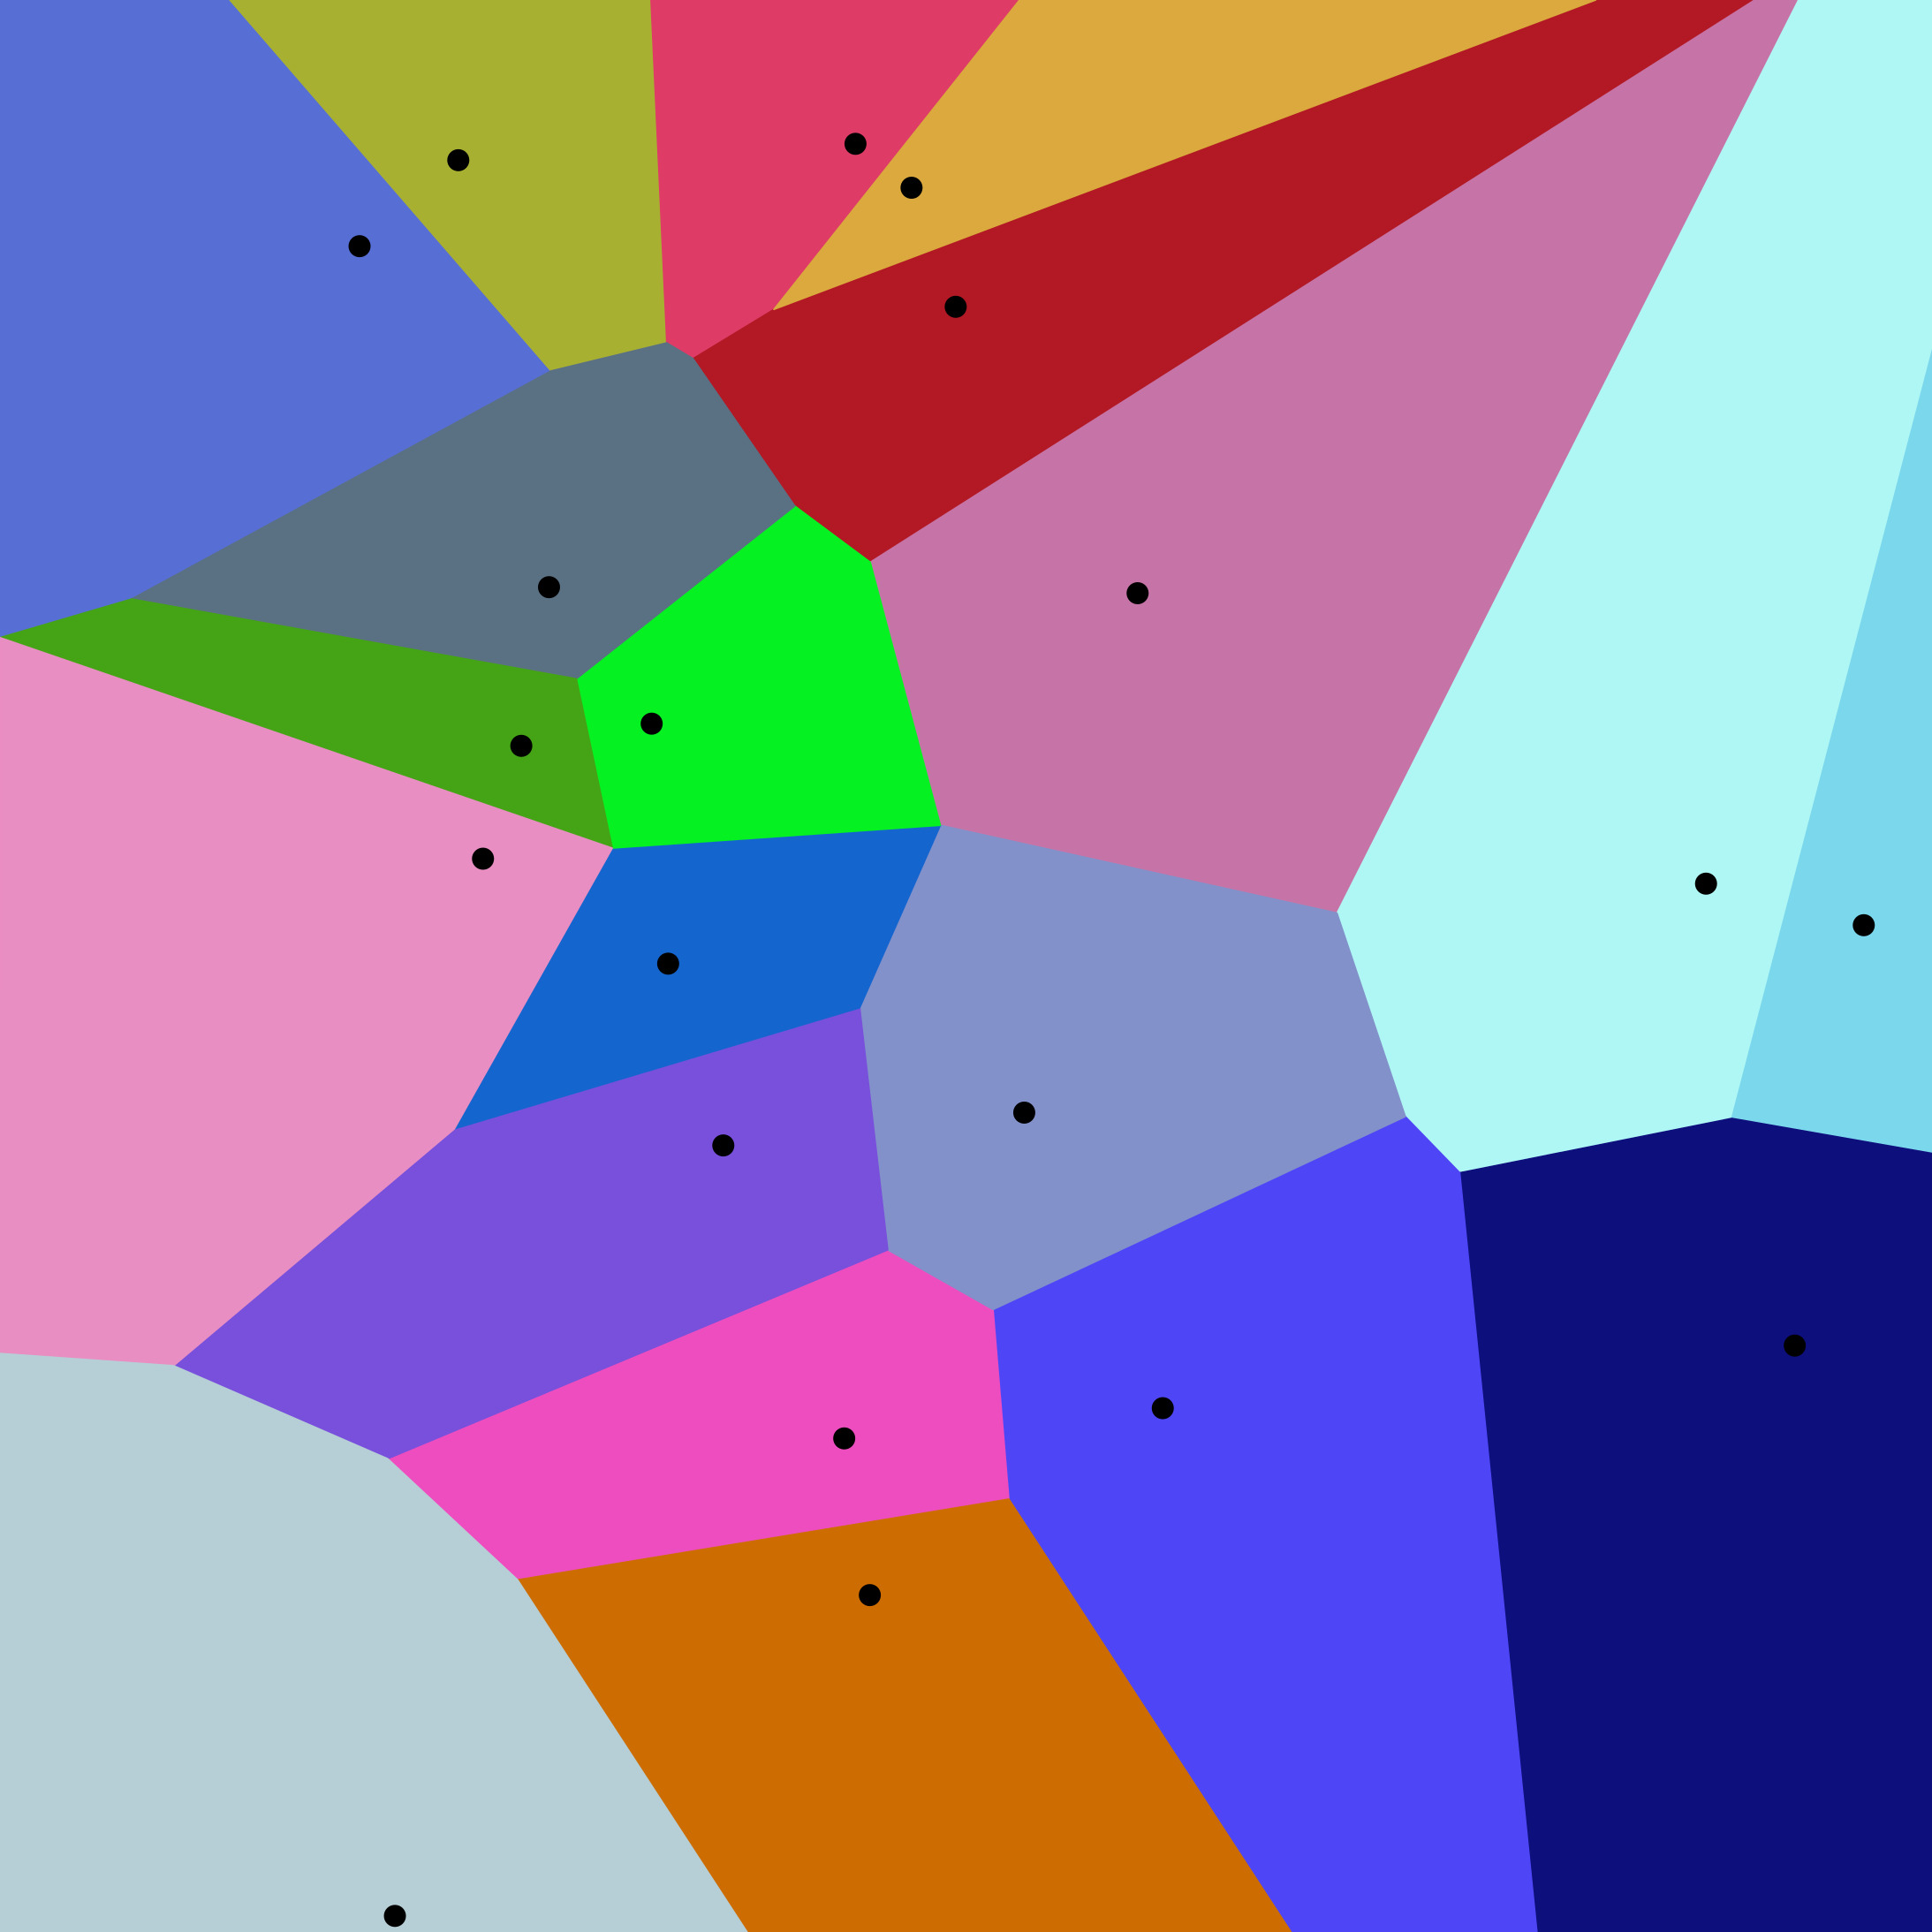
\includegraphics[width=0.48\textwidth, height=0.48\textwidth]{./fig/diagrams/Euclidean_Voronoi_diagram.jpg}
            \label{fig:voronoi_2d}
            }
            \subfloat[Euclidean Voronoi Diagram in 3D] {
            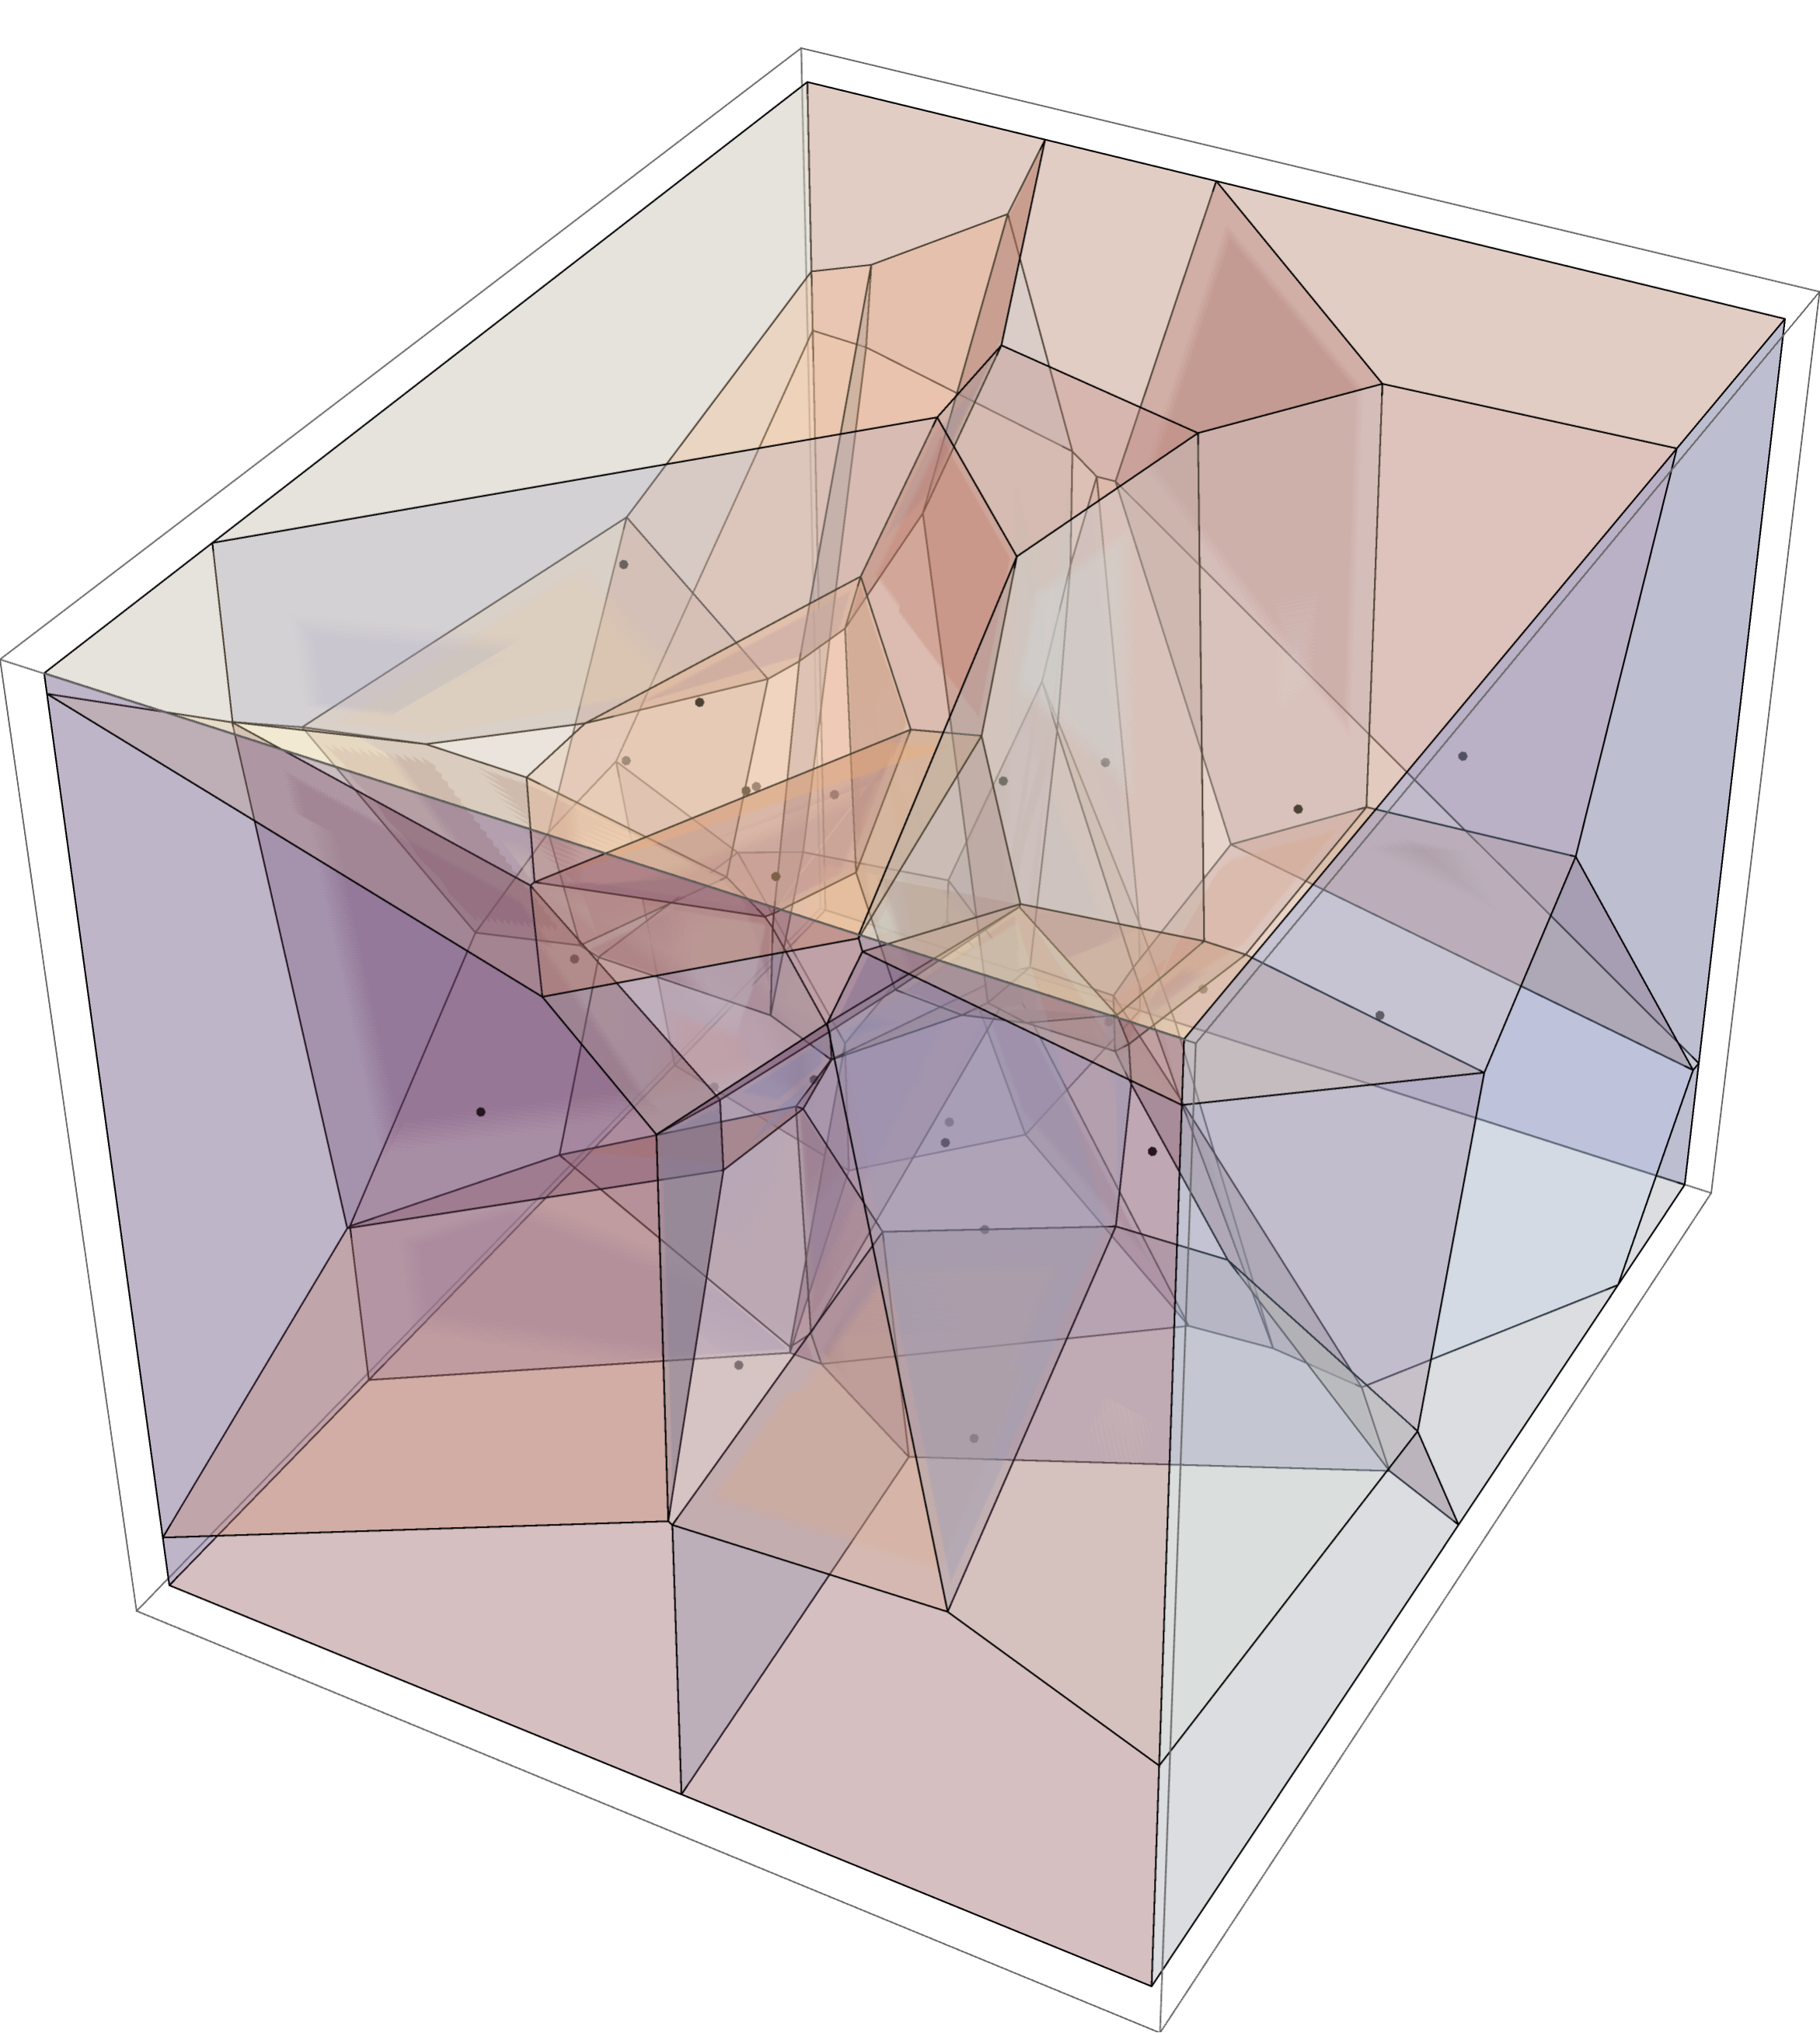
\includegraphics[width=0.48\textwidth, height=0.48\textwidth]{./fig/diagrams/Euclidian Voronoi diagram 3d.png}
            \label{fig:voronoi_3d}
            }
            \caption{
                (a) an example of 20 Voronoi cells in 2D \cite{Voronoi2d} (b) 25 Voronoi cells in 3D \cite{Voronoi3d}
            }
            \label{fig:voronoi_diagrams}
        \end{figure}
    
    \subsection{Additional Constraints and Modifications}
        To extend the approach to the 3D case, several adjustments are made.
        The weighting rule (\ref{eqn:beta_weighting}) remains unchanged. 
        However, in both the azimuth update rule (\ref{eqn:azimuth_2d}) and the azimuth reset rule (\ref{eqn:azimuth_reset_2d}), only the displacement of centroids projected onto the $xy$-plane is taken into account.
        The modified formulations for the 3D case are as follow:
        \begin{itemize}
            \item \textbf{Azimuth update rule 3D}
                \begin{equation}
                    \label{eqn:azimuth_3d}
                    \dot{\theta}_i = 
                    \begin{cases}
                        k  & \text{if } \theta < \frac{\pi}{2} \land \|\mathbf{c}_{\mathcal{A}_i} - \mathbf{c}_{\mathcal{S}_i}\|_{xy} > d_4 \land \|\mathbf{p}_i - \mathbf{c}_{\mathcal{A}_i}\|_{xy} > d_3 \\
                        -k & \text{if } \theta > 0 \land \neg (\|\mathbf{c}_{\mathcal{A}_i} - \mathbf{c}_{\mathcal{S}_i}\|_{xy} > d_4 \land \|\mathbf{p}_i - \mathbf{c}_{\mathcal{A}_i}\|_{xy} > d_3) \\
                        0  & \text{otherwise}
                    \end{cases}
                \end{equation}
            \item \textbf{Azimuth reset rule 3D}
                \begin{equation}
                    \label{eqn:azimuth_reset_3d}
                    \theta = 0 \quad \text{if } \theta = \frac{\pi}{2} \land \| \mathbf{p}_i - \mathbf{\overline{c}}_{\mathcal{A}_i} \|_{xy}    
                \end{equation}
        \end{itemize}

        The notation $\| \cdot \|_{xy}$ denotes the Euclidean norm computed in the $xy$-plane only, defined as:
        \begin{equation}
            \| \mathbf{p}_i - \mathbf{p}_j \|_{xy} = \sqrt{(x_i - x_j)^2 + (y_i - y_j)^2}
        \end{equation}



        Additionally, $Z_{clipping}$ is applied to each sensing cell $\mathcal{S}_i$, constraining it within the vertical limits defined by $\text{min}_z$ and $\text{max}_z$:

        \begin{equation}
            \mathcal{S}_i = \left\{\mathbf{q} \in \mathcal{Q} \mid \|\mathbf{q} - \mathbf{p}_i\| \leq r_{s,i}, \quad \text{min}_z \leq q_z \leq \text{max}_z \right\}
        \end{equation}

        where $\text{min}_z$ and $\text{max}_z$ define the vertical bounds within which the sensing region $\mathcal{S}_i$ is restricted. 
        This ensures that the agent cannot exceed these limits, as it follows the computed centroid \( \mathbf{c}_{V_i} \). 
        By constraining the sensing radius, the agent remains confined within the specified region, preventing it from moving outside the vertical interval $\text{min}_z$ to $\text{max}_z$.

        The destination rotation rule $Z_{rule}$ is introduced to enhance agents avoidance by rotating the computed destination $\mathbf{d}_i$ by an angle $\phi$.
        For vertical rotation angle $\phi$, the following condition is intorduced
        \begin{equation}
            \label{eqn:phi_condition}
            \Omega = \|\mathbf{c}_{\mathcal{A}_i} - \mathbf{c}_{\mathcal{S}_i}\|_z < d_6 \land \|\mathbf{p}_i - \mathbf{c}_{\mathcal{A}_i}\|_z \lor 
            | \|\mathbf{p}_i - \mathbf{c}_{\mathcal{S}_i}\|_{xy} - \|\mathbf{p}_i - \mathbf{c}_{\mathcal{A}_i}\|_{xy} | > d_7
        \end{equation}
        This condition has two main parts, combined by a logical or. The first part evaluates the vertical displacement of the centroid of the partitioned cell $\mathbf{c}_{\mathcal{A}_i}$ from the centroid of the sensing cell $\mathbf{c}_{\mathcal{S}_i}$ and the
        displacement of the agents position $\mathbf{p}_i$ from  $\mathbf{c}_{\mathcal{A}_i}$.
        The second part considers the difference in the horizontal plane between the agent's position and the centroids $\mathbf{c}_{\mathcal{A}_i}$, $\mathbf{c}_{\mathcal{S}_i}$.

        To improve agent distriution in the vertical dimension, a directional influence on vertical exploration is introduced. 
        Given that each agent's position $\mathbf{p}_i$ and final goal $\mathbf{g}_i$, are known, this direc influence can be included into the update rule for $\phi_i$.

        First, the global heading angle, $\theta_{goal}$, towards the goal is calculated: 
        \begin{equation}
            \theta_{goal} = \text{atan2}(g_{i,y} - p_{i,y}, g_{i,x} - p_{i,x})
        \end{equation}
        where $\mathbf{g}_{i, x}$, $\mathbf{g}_{i, y}$ represent the x and y coordinates of the goal, and $\mathbf{p}_{i, x}$, $\mathbf{p}_{i, y}$ represent the x and y coordinates of the agent.
        The resulting angle is in the range $[-\pi, \pi]$.
        Next, the heading angle is linearly mapped to a direction influence $D_{influence}$ value in the range [-1, 1]:
        \begin{equation}
            D_{influence} = \frac{\theta_{goal}}{\pi}
        \end{equation}
        This mapping ensures that agents traveling directly northward (from South to North) have a directional influence close to one, that will promote upward vertical exploration. 
        Similarly, agents traveling southward have a direction influence close to -1, promoting downward exploration. 
        Agents moving primarily eastward or westward have a directional influence close to 0, resulting in minimal vertical exploration.
        This strategy encourages a more uniform distribution of agents throughout the 3D space. 

        To determine the adjustment to the agent's vertical orientation, the directional influence $D_{influence}$ is combined with the relative vertical displacement of the agent and $\mathbf{c}_{\mathcal{S}_i}$
        Weighted average is used to combine them: 
        \begin{equation}
            \label{eqn:combined_influace}
            C_{influence} = \frac{w_1 \cdot (\mathbf{c}_{\mathcal{S}_i,z} - \mathbf{p}_{i,z}) + w_2 \cdot D_{influence}}{w_1 + w_2}
        \end{equation} 
        where $w_1$ $w_2$ are weighting factors. The resulting combined influence $C_{influence}$ is then used to update the agent's rotation of it's destination $\mathbf{d}_i$ by $\phi_i$.

        Based on condition \eqref{eqn:phi_condition} and \eqref{eqn:combined_influace} update rule for $phi_i$ can be constructed as follows:
        \begin{equation}
            \label{eqn:phi_update}
            \dot{\phi}_i = 
            \begin{cases}
                k  & \text{if } \phi_i < \frac{\pi}{4} > \land C_{influence} > 0 \land \Omega \\
                0  & \text{if } \phi_i > \frac{\pi}{4} > \land C_{influence} > 0 \land \Omega \\
                -k & \text{if } \phi_i > -\frac{\pi}{4} > \land C_{influence} \leq 0 \land \Omega \\
                0  & \text{if } \phi_i < -\frac{\pi}{4} > \land C_{influence} \leq 0 \land \Omega \\
                -k & \text{if } \phi_i > 0 \land \neg \Omega \\
                k  & \text{if } \phi_i < 0 \land \neg \Omega \\
                0  & \text{otherwise}
            \end{cases}
        \end{equation}
        where the first four cases control the rotation of the agent's destination $\mathbf{d}_i$ and the final three cases handle the smooth convergence of $\phi_i$ back to 0, when the condition $\Omega$ is not met. 

        After the application of the rules for $\theta_i$ and $\phi_i$, the agent's destination is updated as:
        \begin{equation}
            \label{eqn:destination_update}
            \mathbf{d}_i =
            \begin{pmatrix}
                p_{i,x} +  \|\mathbf{p}_i - \mathbf{g}_i\| \cdot \sin(\phi_{\mathbf{g}_i} + \phi_i) \cdot \cos(\theta_{\mathbf{g}_i} - \theta_i) \\
                p_{i,y} + \|\mathbf{p}_i - \mathbf{g}_i\| \cdot \sin(\phi_{\mathbf{g}_i} + \phi_i) \cdot \sin(\theta_{\mathbf{g}_i} - \theta_i) \\
                p_{i,z} + \|\mathbf{p}_i - \mathbf{g}_i\| \cdot \cos(\phi_{\mathbf{g}_i} + \phi_i)
            \end{pmatrix}
        \end{equation}

        where $\phi_{\mathbf{g}_i} = \arccos(\frac{\mathbf{g}_{i,z} - \mathbf{p}_{i,z}}{\|\mathbf{p}_i - \mathbf{g}_i\|})$ is the polar angle from z-axis to the goal, 
        $\theta_{\mathbf{g}_i} = atan2( \mathbf{g}_{i,y} - \mathbf{p}_{i,y}, \mathbf{g}_{i,x} - \mathbf{p}_{i,x})$ is the azimuthal angle in the xy-plane to the goal.
    
    \subsection{Algorithm Walkthrough}
        At each iteration, the proposed algorithm performs a sequence of actions to control agent movement. 
        These actions can be summarized as follows:
        \begin{enumerate}
            \item \textbf{Cell Generation:} \\
                For each agent, two cells are generated: a partitioned cell, denoted as '$\mathcal{A}$' and a sensing cell, denoted as '$\mathcal{S}$'.
            \item \textbf{Centroid Computation:}
                \begin{itemize}
                    \item The centroid of cell $\mathcal{A}$, $c_{\mathcal{A}}$ is computed using a weighted function that considers both the agent's goal position, $\mathbf{g}_i$, and its current destination, $\mathbf{d}_i$.
                    \item The centroid of cell $\mathcal{S}$, $c_{\mathcal{S}}$ is computed using a weighted function that considers only the agent's current destination, $\mathbf{d}_i$.
                \end{itemize}
            \item \textbf{Rule Application and Destination Update:} \\
                A set of rules is applied to: 
                \begin{itemize}
                    \item Adjust weighting function usied in the centroid computations \eqref{eqn:beta_weighting}.
                    \item Rules to update $\theta_i$ \eqref{eqn:azimuth_3d} and $\phi_i$ \eqref{eqn:phi_update} are applied.
                    \item Update the agent's destination $\mathbf{d}_i$ \eqref{eqn:destination_update}.
                \end{itemize}
            \item \textbf{Agent movement} \\
                Finally, the agent is directed towards a centroid location $c_{\mathcal{A}}$.
        \end{enumerate}
        This process is repeated until all agents reach their goals.

        

\section{Simulation and Results Analysis}

    \subsection{Computational Implementation Details}
        The continuous algorithm presented in the previous section can be easily discretized for implementation in a computational enviroment.
        Instead of continuous sets, the cells $\mathcal{A}$ and $\mathcal{S}$ are aproximated using a set of discrete points.   
        Discrete points are partitioned out when definition \eqref{eq:voronoi_cell_account_encum} is not met.
        \begin{figure}[H]
            \centering
            \subfloat[Example of discretized cells ($\mathcal{A} = \mathcal{S}$)] {
            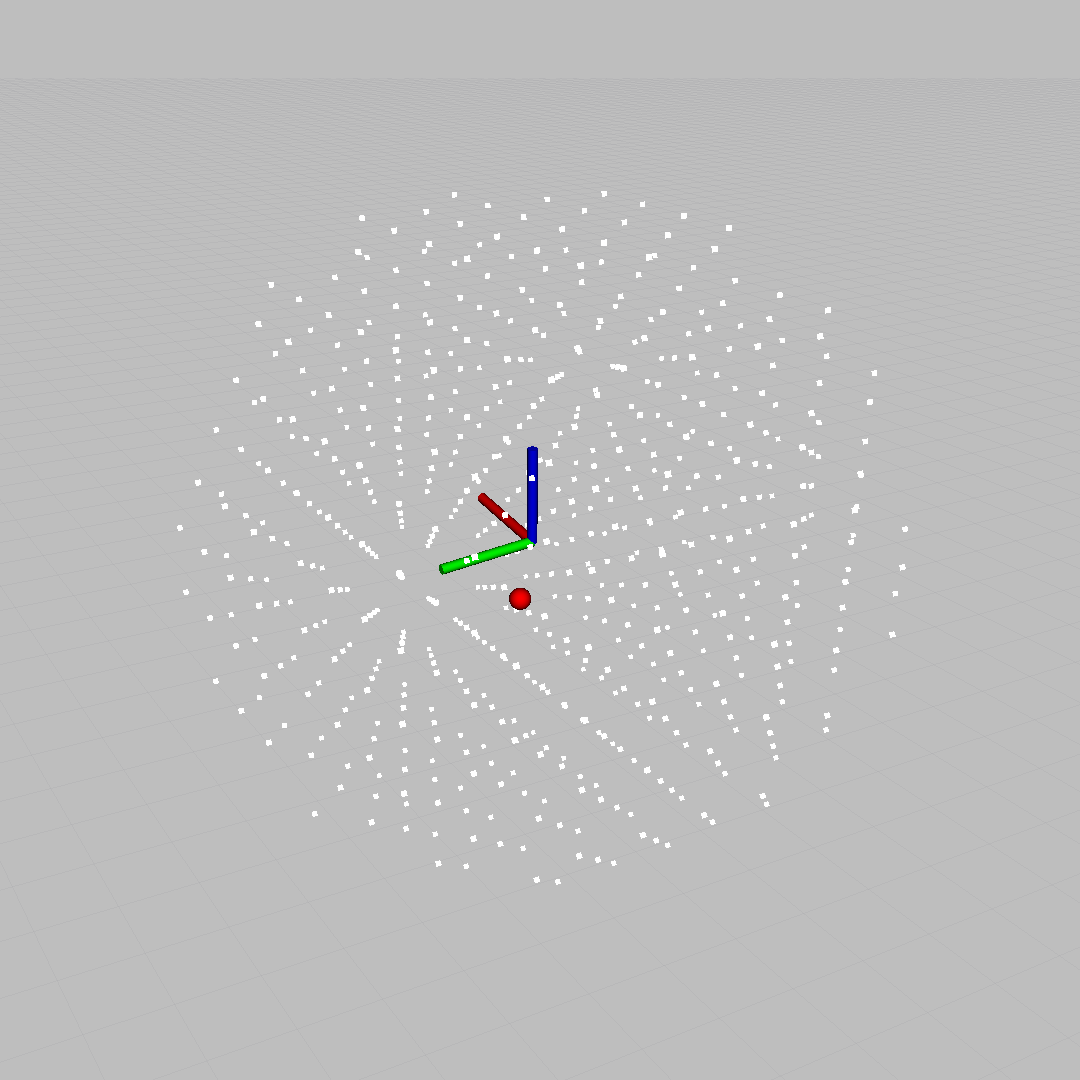
\includegraphics[width=0.48\textwidth, height=0.48\textwidth]{./fig/rviz/cs_equal_ca.png}
            \label{fig:rviz_cs_eq_ca}
            }
            \subfloat[Example of a partitioned cell $\mathcal{A}$] {
            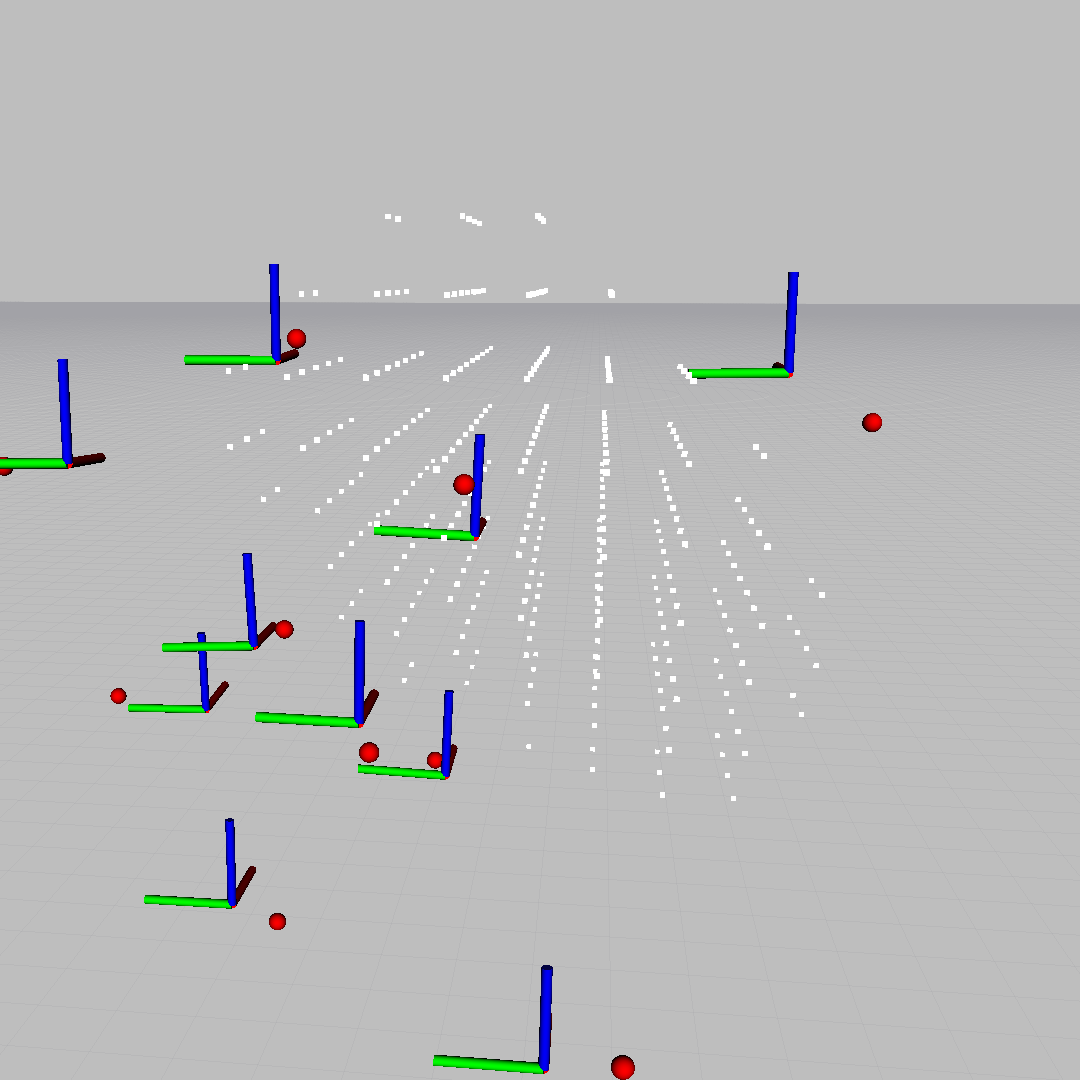
\includegraphics[width=0.48\textwidth, height=0.48\textwidth]{./fig/rviz/ca_partitioned.png}
            \label{fig:rviz_ca_partitioned}
            }
            \caption{
                Discrete approximation of Voronoi cells, with centroid $c_{\mathcal{A}}$ shown as a red dot.(a) Example where the partitioned cell $\mathcal{A}$ and the sensing cell $\mathcal{S}$ are the same. (b) Example where the partitioned cell $\mathcal{A}$ is partitioned by other \ac{UAV}s.
            }
            \label{fig:rviz_cells}
        \end{figure}
        
    \subsection{Simulation Enviroment}
        In this simulation, the term 'agent' refers to the \ac{UAV}, which were simulated using the framework provided by \cite{mrs_uav_system}.
        Each \ac{UAV} obtains its global ground truth position from the ROS simulator.
        The positions of neighboring \ac{UAV}s were estimated using simulated blinking ultraviolet markers, following the method described in \cite{uvdd1} and \cite{uvdar_package}.
        The following constraints are relevant for each \ac{UAV}:
        \begin{table}[h]
            \centering
            \renewcommand{\arraystretch}{1.1}
            \begin{tabular}{|l|c|}
                \hline
                \textbf{Parameter} & \textbf{Value} \\ \hline
                    Maximal horizontal velocity [\SI{}{\meter\per\second}] & 4.0 \\ \hline
                    Horizontal acceleration [\SI{}{\meter\per\second\squared}] & 2.0 \\ \hline
                    Maximal ascending velocity [\SI{}{\meter\per\second}] & 2.0 \\ \hline
                    Vertical ascending acceleration [\SI{}{\meter\per\second\squared}] & 1.0 \\ \hline
                    Maximal descending velocity [\SI{}{\meter\per\second}] & 2.0 \\ \hline
                    Vertical descending acceleration [\SI{}{\meter\per\second\squared}] & 1.0 \\ \hline
                \end{tabular}
                \caption{Motion constraints of the \ac{UAV}.}
            \label{tab:uav_constraints}
        \end{table}
        
    \subsection{Simulation Scenarios}
        To evaluate the safety and performance of the \ac{UAV}s during interactions, a series of experiments was conducted. 
        Experiments were performed primarily using circular formations, with \ac{UAV} counts of N = 5, 10, and 15. 
        Each of these circular formation experiments was repeated 10 times.
        Additionally, to extend the analysis to 3D and assess the algorithm's performance, a set of spherical formation experiments eas conducted with N = 10, also repeated 10 times.
        After each \ac{UAV} was flown from the ground to its designated starting position, the \ac{RBL} algorithm was initiated.    

        These formations provide a controlled enviroment compared to random initial position and goal locations. 
        In both circular and spherical formations, the \ac{UAV}s were evenly distributed along the circle or the surface of the sphere, with the goal position located on the opposite side.
        The radius of both circle and the sphere was set to 5 meters.
        
        The following metrics were measured across the 10 repetitions of each experiment, along with their standard deviations: success rate \( SR \ [\%] \), average trajectory length \( \overline{L} \ [\mathrm{m}] \), 
        average time to reach the goal \( \overline{t} \ [\mathrm{s}] \), average of the maximal time for \ac{UAV} to reach the goal \( \overline{t}_{\text{max}} \ [\mathrm{s}] \), and average velocity \( \overline{v} \ [\mathrm{m/s}] \).

        The specific values of the parameters used in the experiments are summarized in following table \ref{tab:experiment_parameters}:
        \begin{table}[H]
            \centering
            \caption{Parameters Used in Experiments}
            \begin{tabular}{|l|l|}
                \hline
                Parameter & Value \\
                \hline
                \hline
                Sensing radius ($r_s$) & 3.5 m \\ \hline
                Update rate & 10 Hz \\ \hline
                Encumbrance & 0.5 m \\ \hline
                $d_1 = d_3 = d_5$ & 0.5 m \\ \hline
                $d_2 = d_4 = d_6$ & 1.0 m \\ \hline
                $d_7$ & 0.2  \\ \hline
                $\beta_i^D$ & 1.5  \\ \hline
                $\eta$ & 0.9  \\ \hline
                $min_z$ & 1.0 m \\ \hline
                $max_z$ & 10.0 m \\ \hline

            \end{tabular}
            \label{tab:experiment_parameters}
        \end{table}

    \subsection{Experimental Results}
        \begin{itemize}
            \item \textbf{$N = 5$ Circular Formation:}
                \begin{table}[H]
                    \centering
                    \renewcommand{\arraystretch}{1.2}
                    \begin{tabular}{|l|c|c|c|c|c|}
                    \hline
                                                & \( SR \ [\%] \) & \( \overline{L} \ [\mathrm{m}] \) & \( \overline{t} \ [\mathrm{s}] \) & \( \overline{t}_{\text{max}} \ [\mathrm{s}] \) & \( \overline{v} \ [\mathrm{m/s}] \)     \\ \hline
                    RBL 2D                      & 100.00          & 21.06 $\pm$ 0.10                  & 25.15 $\pm$ 0.21                  & 25.15 $\pm$ 0.19                               & 0.83 $\pm$ 0.01                         \\ \hline
                    RBL 3D                      & 100.00          & 20.77 $\pm$ 0.29                  & 26.04 $\pm$ 0.51                  & 26.79 $\pm$ 0.27                               & 0.79 $\pm$ 0.02                         \\ \hline
                    RBL 3D\(_{\text{clipped}}\) & 100.00          & 20.60 $\pm$ 0.24                  & 26.73 $\pm$ 0.47                  & 27.39 $\pm$ 0.28                               & 0.77 $\pm$ 0.02                         \\ \hline
                    RBL 3D\(_z\)                & 100.00          & 20.97 $\pm$ 0.52                  & 25.54 $\pm$ 0.97                  & 26.72 $\pm$ 0.60                               & 0.81 $\pm$ 0.03                         \\ \hline
                    \end{tabular}
                \end{table}
            \item \textbf{$N = 10$ Circular Formation:}
                \begin{table}[H]
                    \centering
                    \renewcommand{\arraystretch}{1.2}
                    \begin{tabular}{|l|c|c|c|c|c|}
                    \hline
                                                & \( SR \ [\%] \) & \( \overline{L} \ [\mathrm{m}] \) & \( \overline{t} \ [\mathrm{s}] \) & \( \overline{t}_{\text{max}} \ [\mathrm{s}] \) & \( \overline{v} \ [\mathrm{m/s}] \)     \\ \hline
                    RBL 2D                      & 100.00          & 22.95 $\pm$ 1.64                  & 30.79 $\pm$ 2.28                  & 34.73 $\pm$ 0.77                               & 0.74 $\pm$ 0.07                         \\ \hline
                    RBL 3D                      & 100.00          & 22.22 $\pm$ 0.89                  & 30.05 $\pm$ 2.61                  & 34.39 $\pm$ 4.19                               & 0.73 $\pm$ 0.05                         \\ \hline
                    RBL 3D\(_{\text{clipped}}\) & 100.00          & 22.31 $\pm$ 0.69                  & 30.22 $\pm$ 1.83                  & 33.22 $\pm$ 0.93                               & 0.73 $\pm$ 0.04                         \\ \hline
                    RBL 3D\(_z\)                & 100.00          & 22.38 $\pm$ 0.88                  & 28.80 $\pm$ 2.30                  & 32.35 $\pm$ 1.25                               & 0.77 $\pm$ 0.05                         \\ \hline
                    \end{tabular}
                \end{table}
            \item \textbf{$N = 15$ Circular Formation:}
                \begin{table}[H]
                    \centering
                    \renewcommand{\arraystretch}{1.2}
                    \begin{tabular}{|l|c|c|c|c|c|}
                    \hline
                                                & \( SR \ [\%] \) & \( \overline{L} \ [\mathrm{m}] \) & \( \overline{t} \ [\mathrm{s}] \) & \( \overline{t}_{\text{max}} \ [\mathrm{s}] \) & \( \overline{v} \ [\mathrm{m/s}] \)     \\ \hline
                    RBL 2D                      & 100.00          & 23.56 $\pm$ 1.75                  & 33.89 $\pm$ 2.48                  & 38.75 $\pm$ 1.45                               & 0.69 $\pm$ 0.06                         \\ \hline
                    RBL 3D                      & 100.00          & 22.36 $\pm$ 0.97                  & 30.65 $\pm$ 3.07                  & 35.77 $\pm$ 3.72                               & 0.72 $\pm$ 0.07                         \\ \hline
                    RBL 3D\(_{\text{clipped}}\) & 100.00          & 22.32 $\pm$ 0.81                  & 30.69 $\pm$ 2.61                  & 34.50 $\pm$ 0.47                               & 0.72 $\pm$ 0.06                         \\ \hline
                    RBL 3D\(_z\)                & 100.00          & 22.64 $\pm$ 0.95                  & 29.67 $\pm$ 2.54                  & 34.27 $\pm$ 0.88                               & 0.76 $\pm$ 0.06                         \\ \hline
                    \end{tabular}
                \end{table}
            \item \textbf{$N = 10$ Spherical Formation:}
                \begin{table}[H]
                    \centering
                    \renewcommand{\arraystretch}{1.2}
                    \begin{tabular}{|l|c|c|c|c|c|}
                    \hline
                                                & \( SR \ [\%] \) & \( \overline{L} \ [\mathrm{m}] \) & \( \overline{t} \ [\mathrm{s}] \) & \( \overline{t}_{\text{max}} \ [\mathrm{s}] \) & \( \overline{v} \ [\mathrm{m/s}] \)     \\ \hline
                    RBL 3D                      & 100.00          & 14.32 $\pm$ 1.52                  & 27.76 $\pm$ 3.06                  & 32.48 $\pm$ 2.26                               & 0.51 $\pm$ 0.05                         \\ \hline
                    RBL 3D\(_z\)                & 100.00          & 14.06 $\pm$ 0.97                  & 27.17 $\pm$ 2.66                  & 31.86 $\pm$ 1.24                               & 0.55 $\pm$ 0.06                         \\ \hline
                    \end{tabular}
                \end{table}
        \end{itemize}

        The figure below visualizes the  \ac{UAV}  trajectories, showing the effect of the applied simulation rules.
        \begin{figure}[H]
            \centering
            \subfloat[Trajectories of \ac{UAV}s using 2D \ac{RBL}, $N=10$] {
                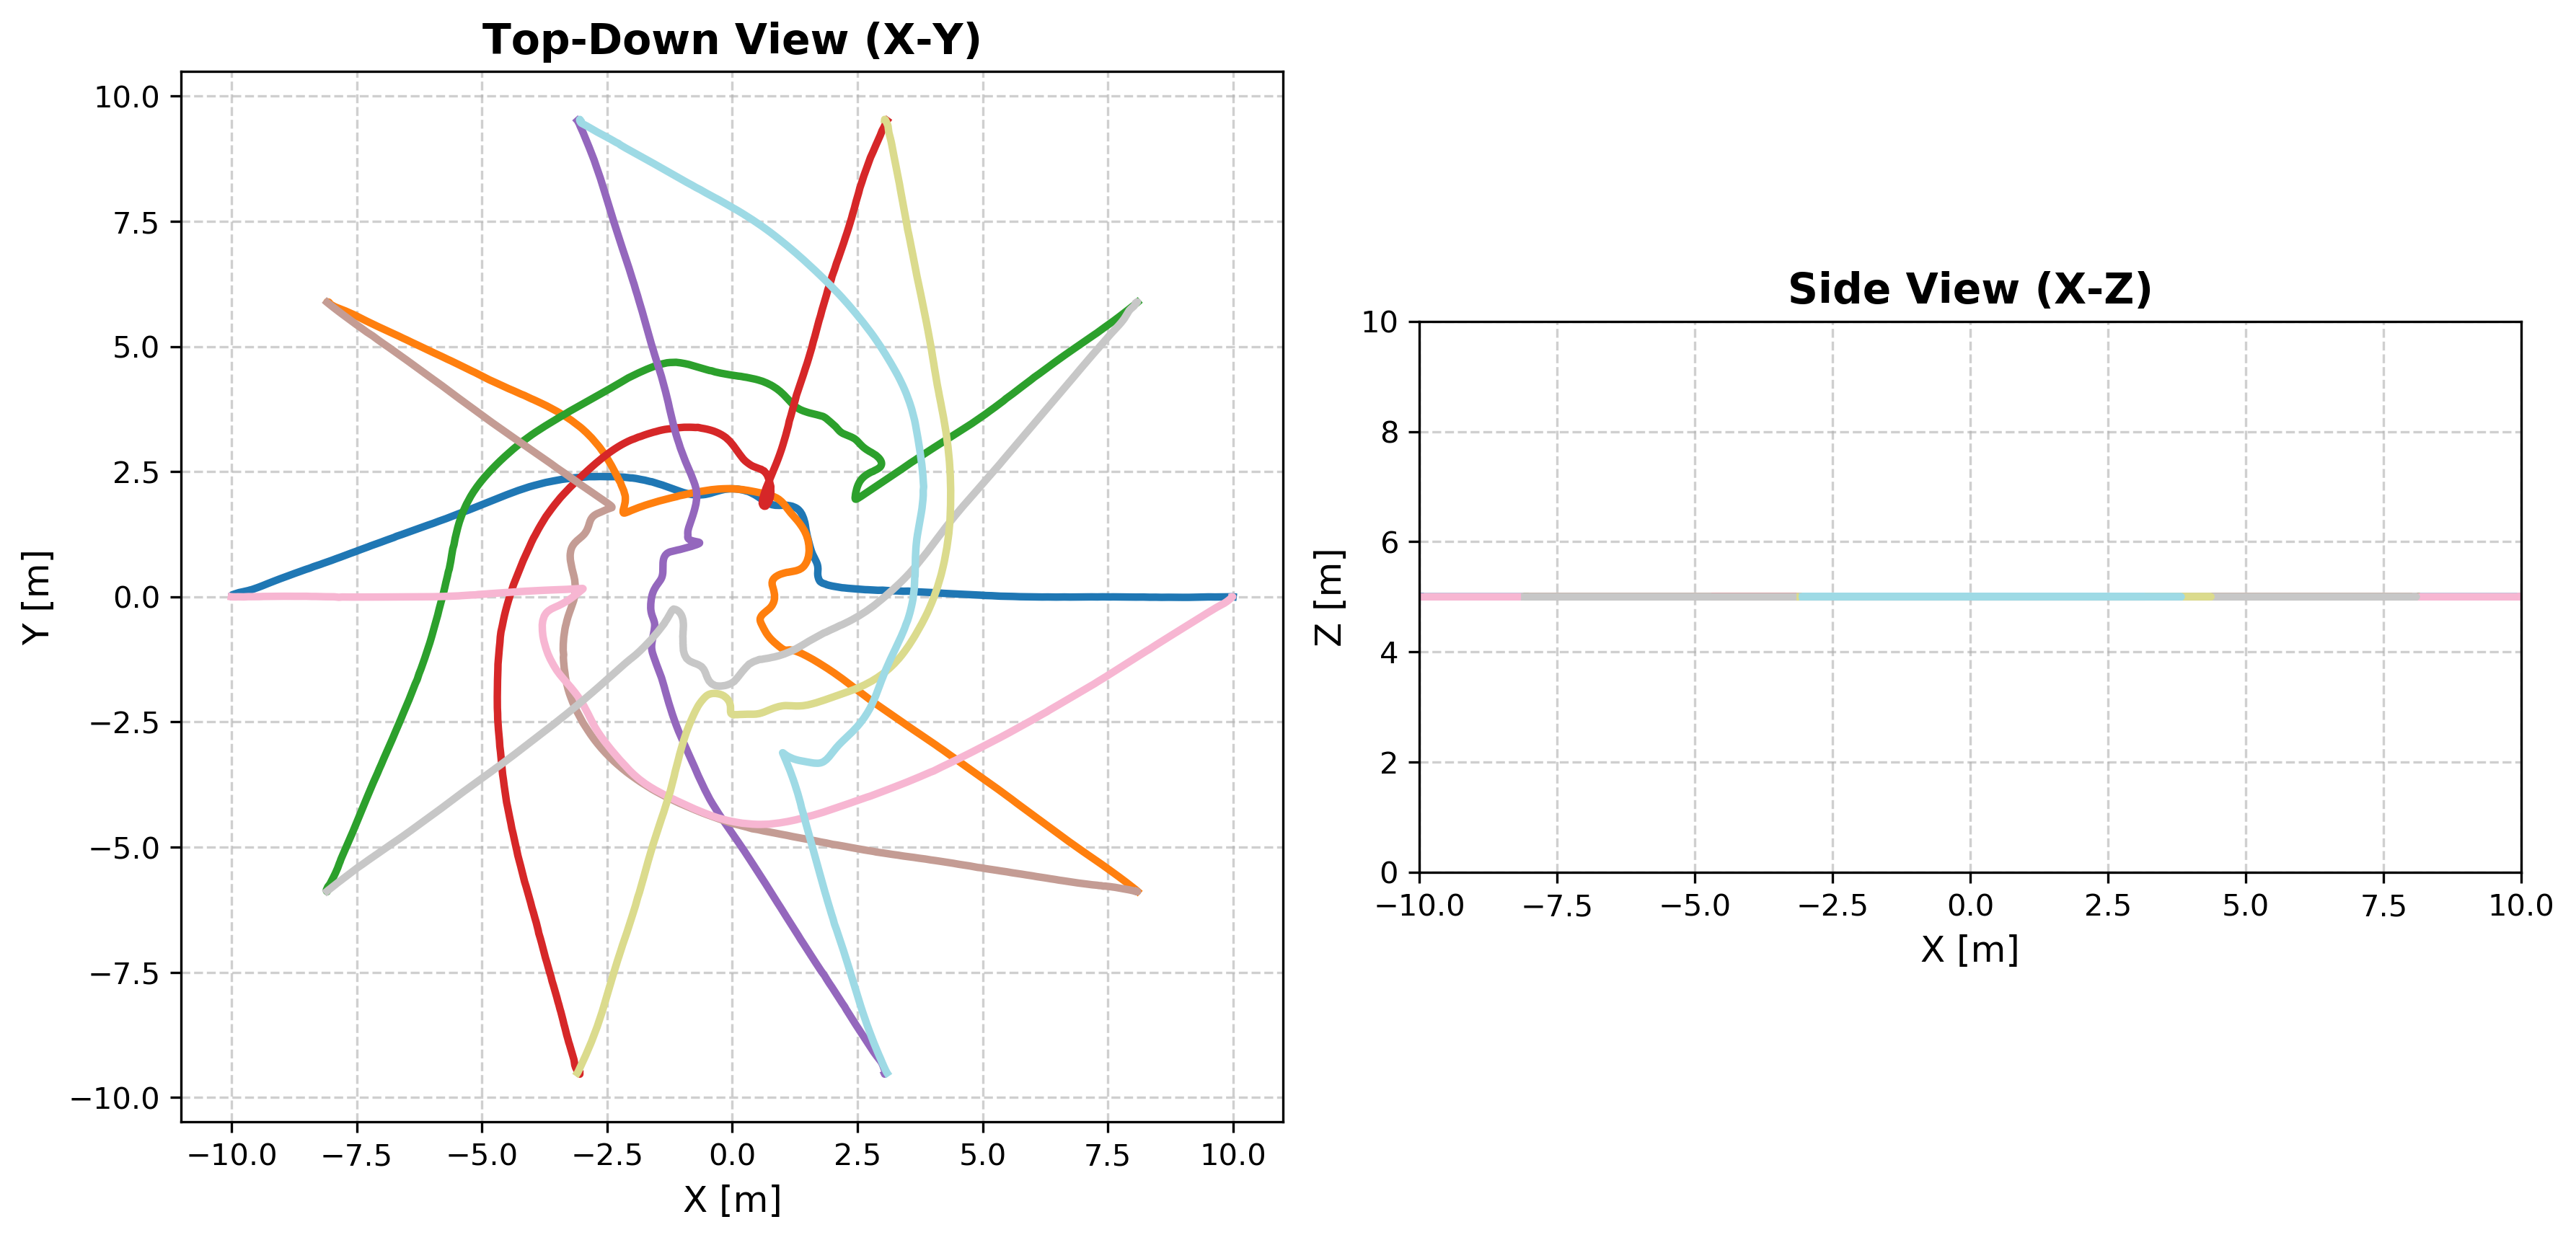
\includegraphics[width=0.48\textwidth, height=0.24\textwidth]{./fig/plots/n_10_circle_2d.png}
                \label{fig:n_10_circle_2d}
            }
            \subfloat[Trajectories of \ac{UAV}s using 3D \ac{RBL}, $N=10$] {
                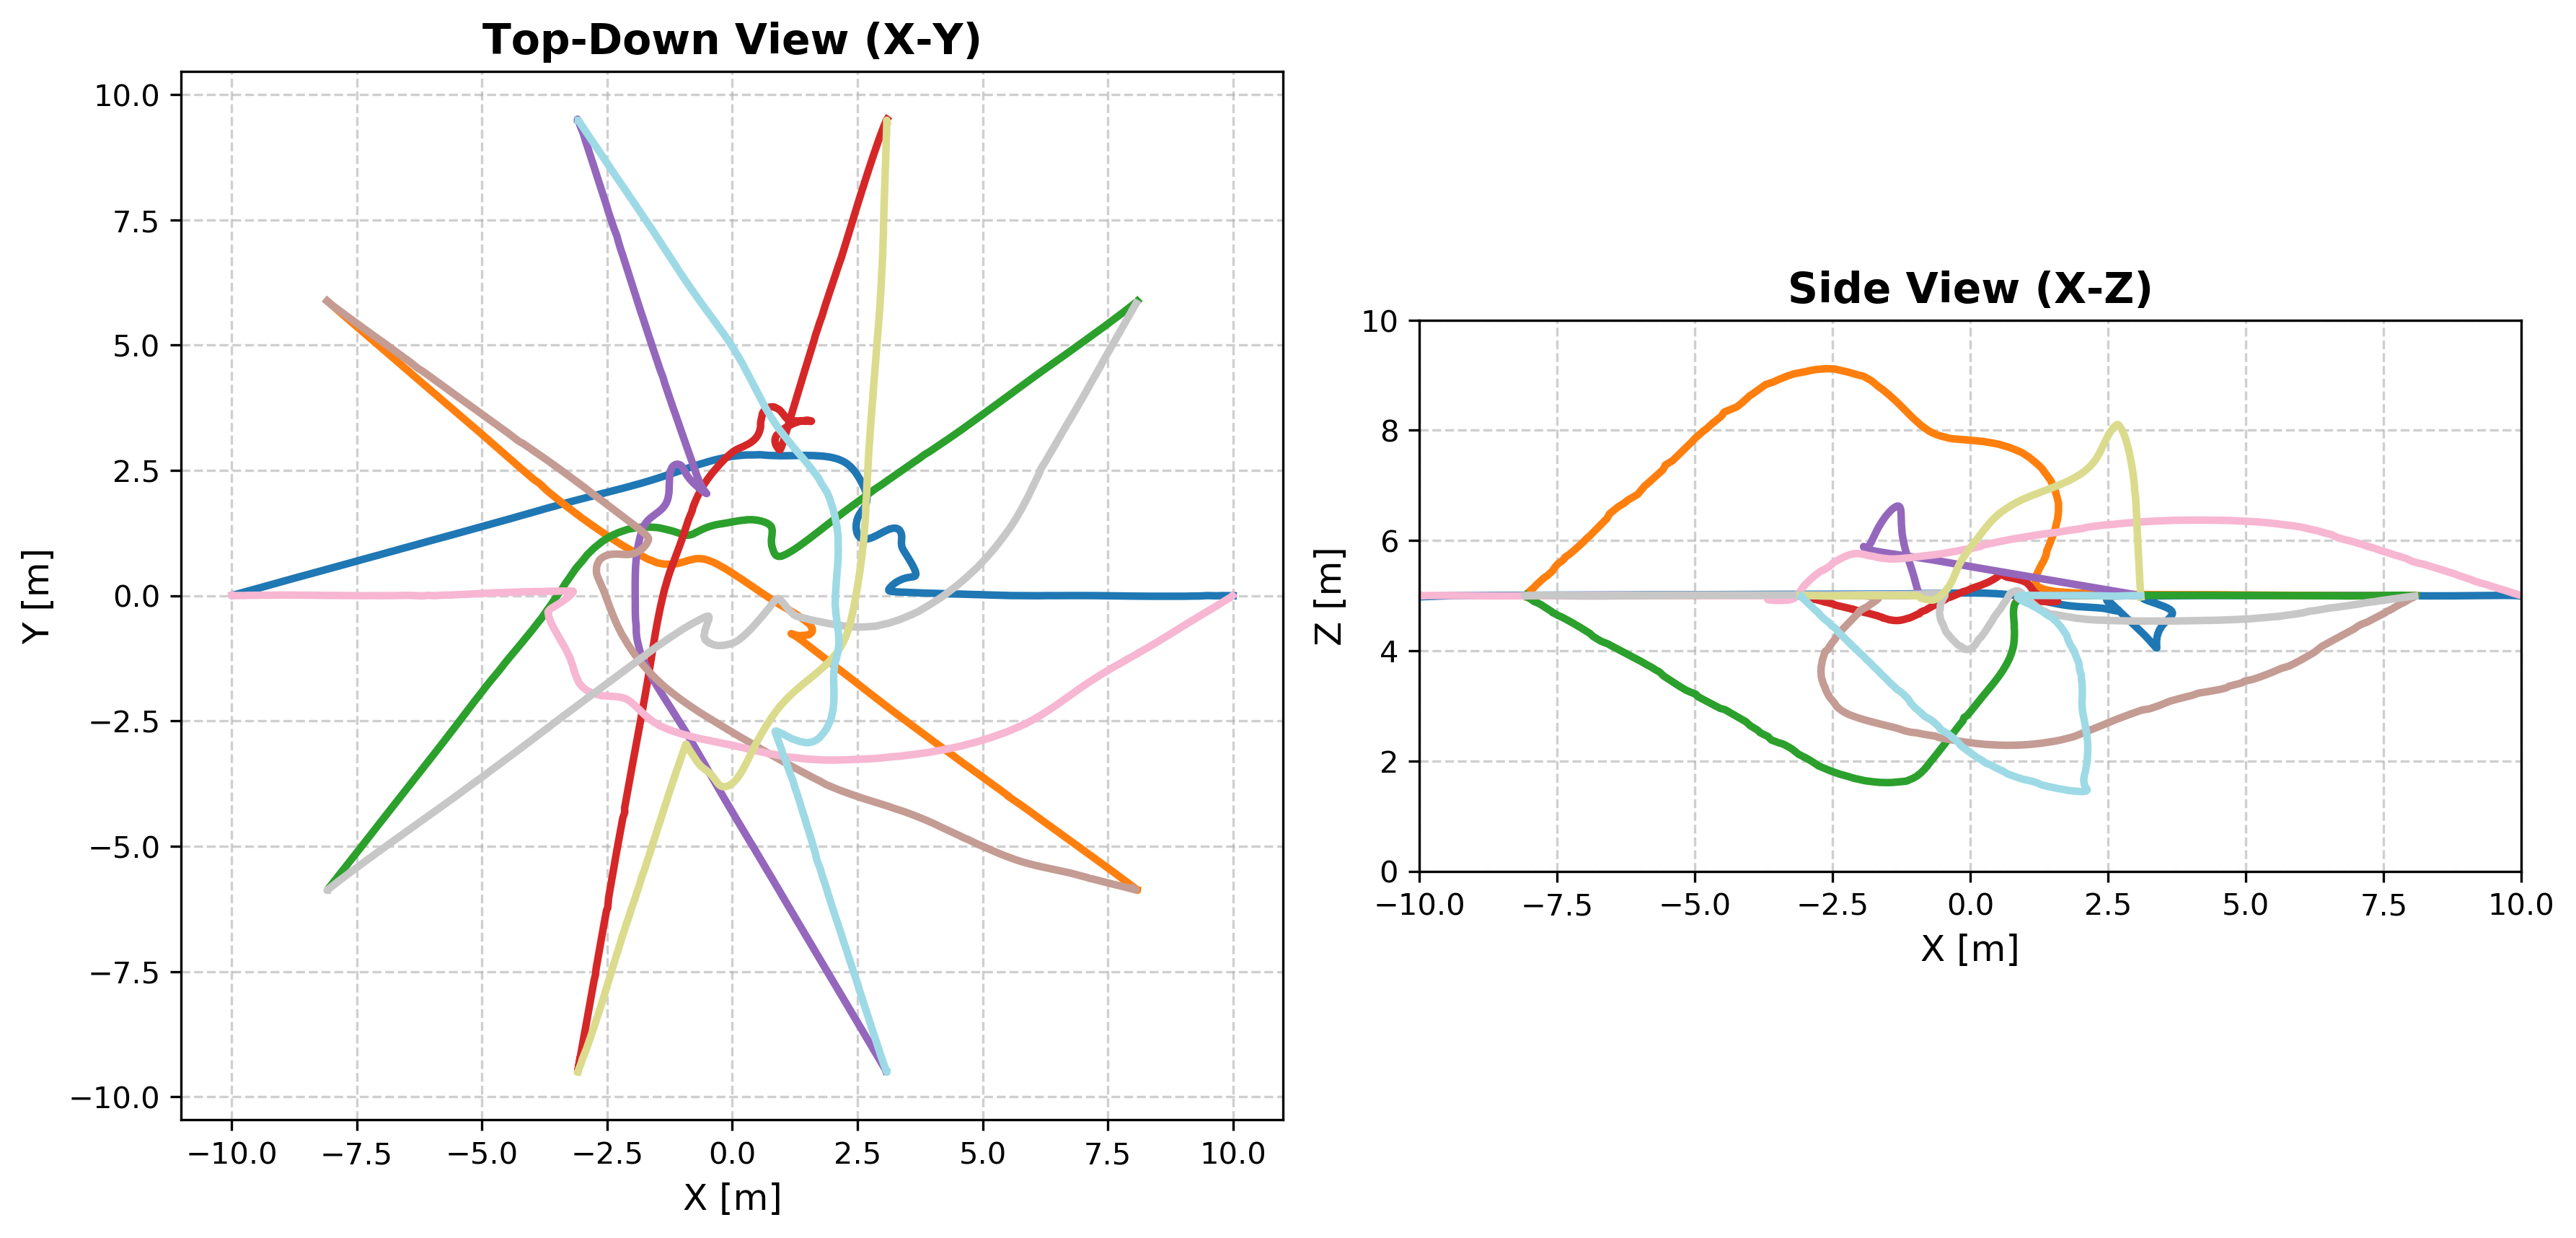
\includegraphics[width=0.48\textwidth, height=0.24\textwidth]{./fig/plots/n_10_circle_3d.png}
                \label{fig:n_10_circle_3d}
            }
            \par\medskip
            \subfloat[Trajectories of \ac{UAV}s using 3D \ac{RBL} and $Z_{clipping}$, $N=10$] {
                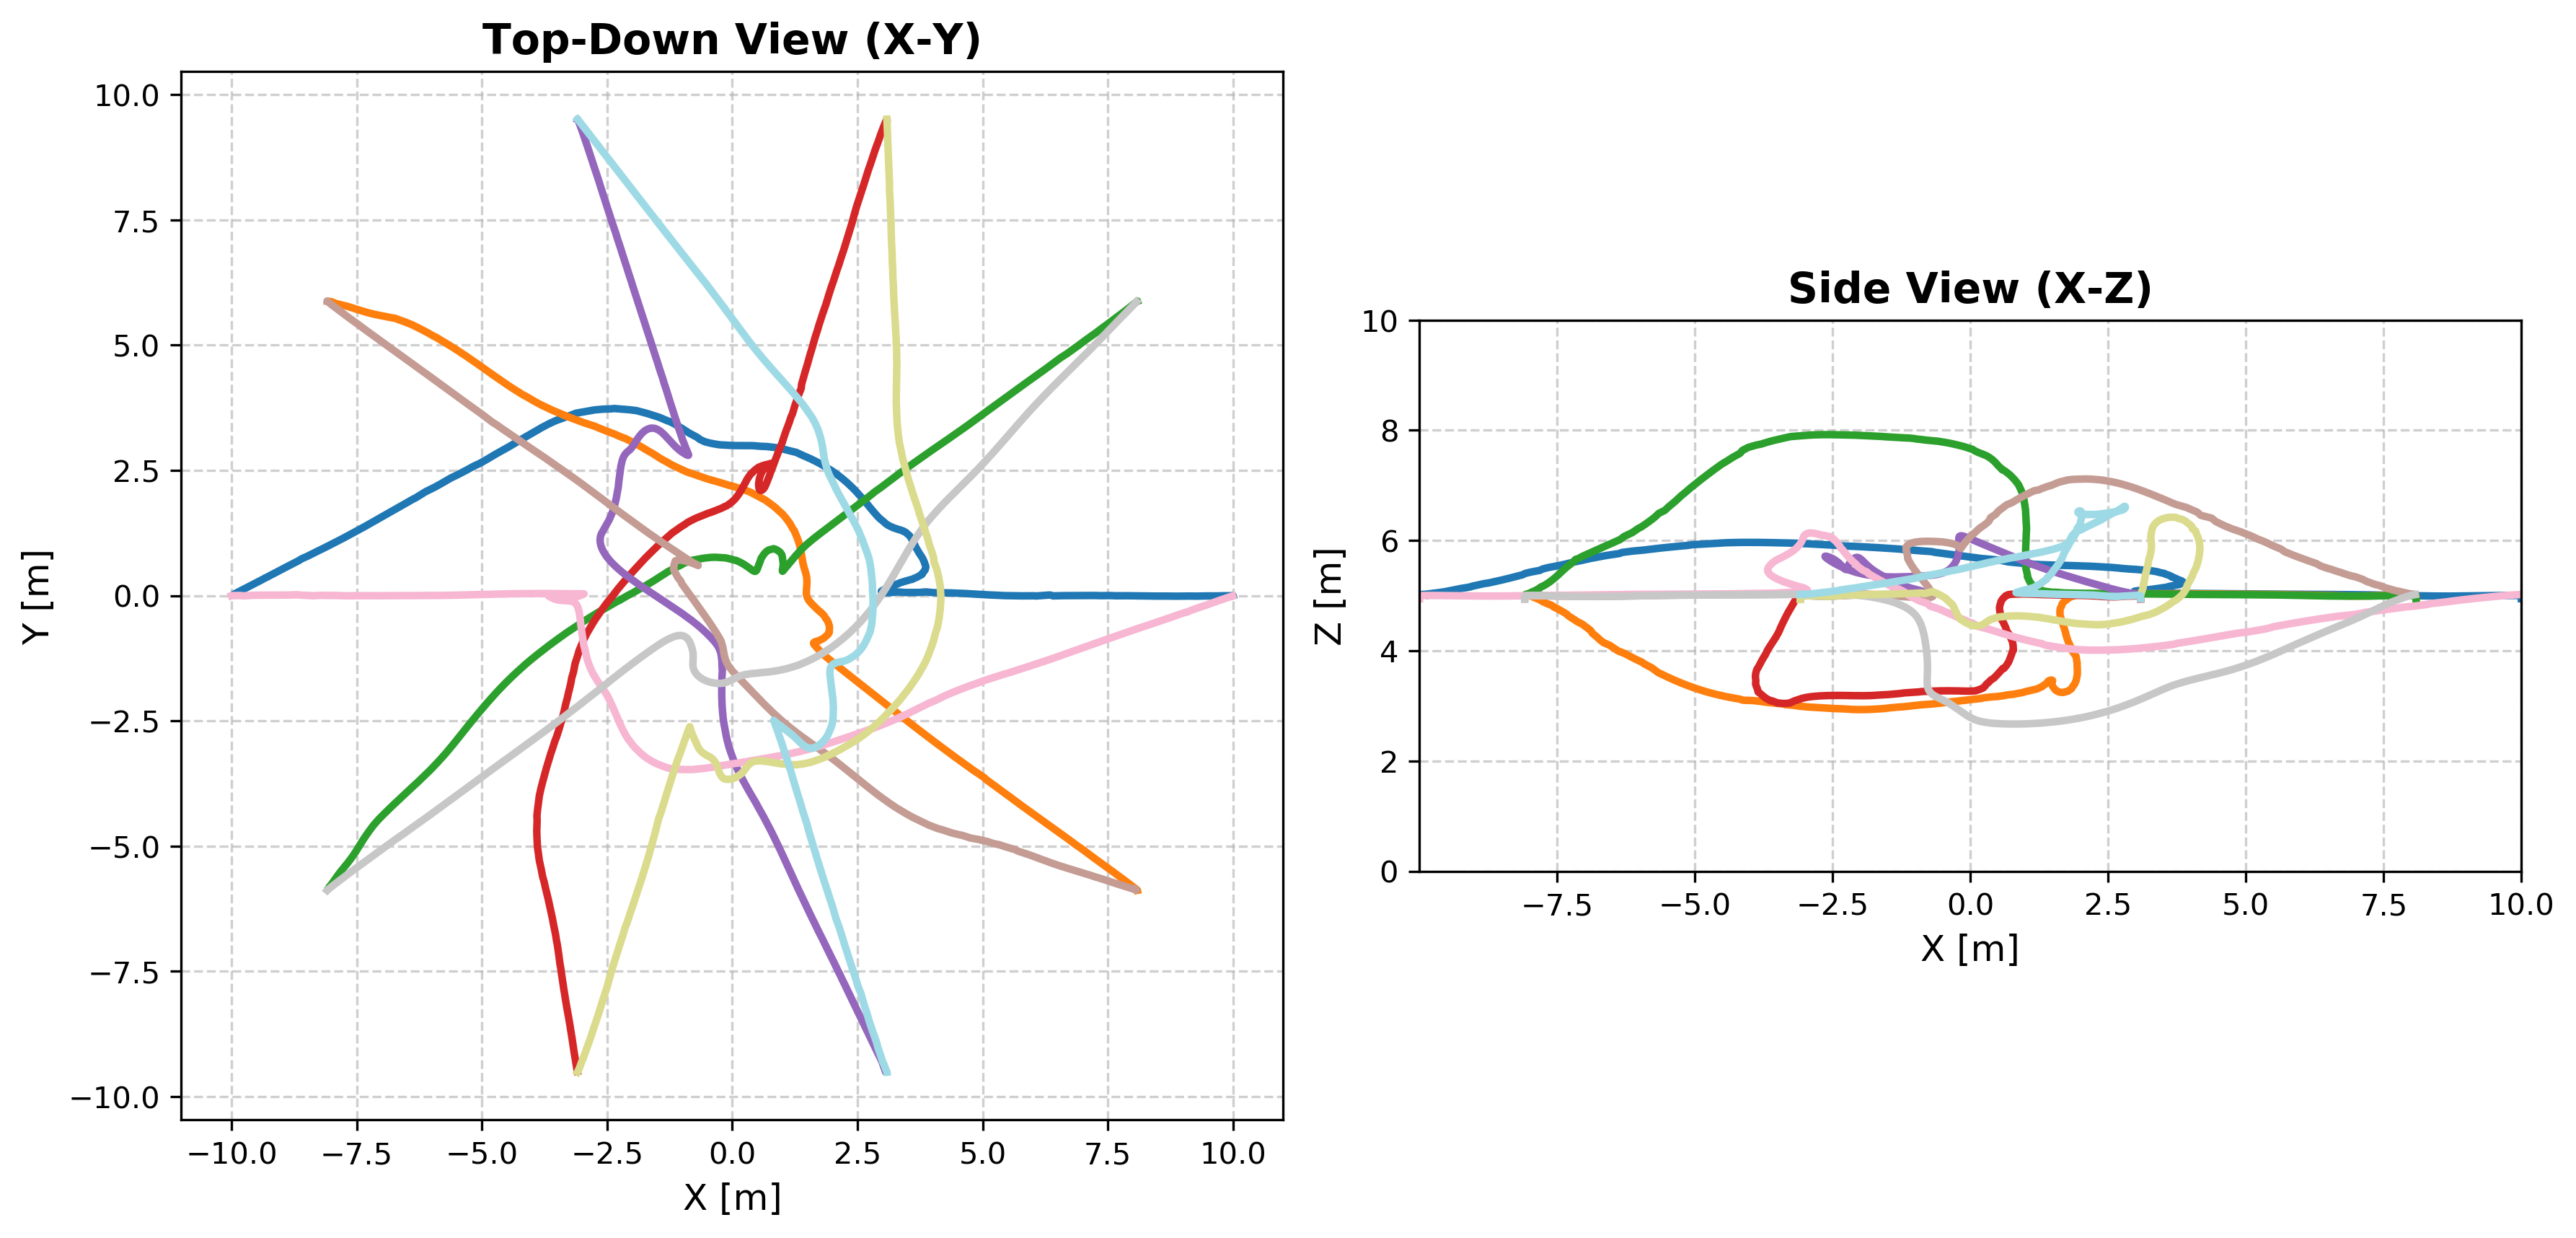
\includegraphics[width=0.48\textwidth, height=0.24\textwidth]{./fig/plots/n_10_circle_z_clipp.png}
                \label{fig:n_10_circle_z_clipp}
            }
            \subfloat[Trajectories of \ac{UAV}s using 3D \ac{RBL} and using $Z_{rule}$, $N=10$] {
                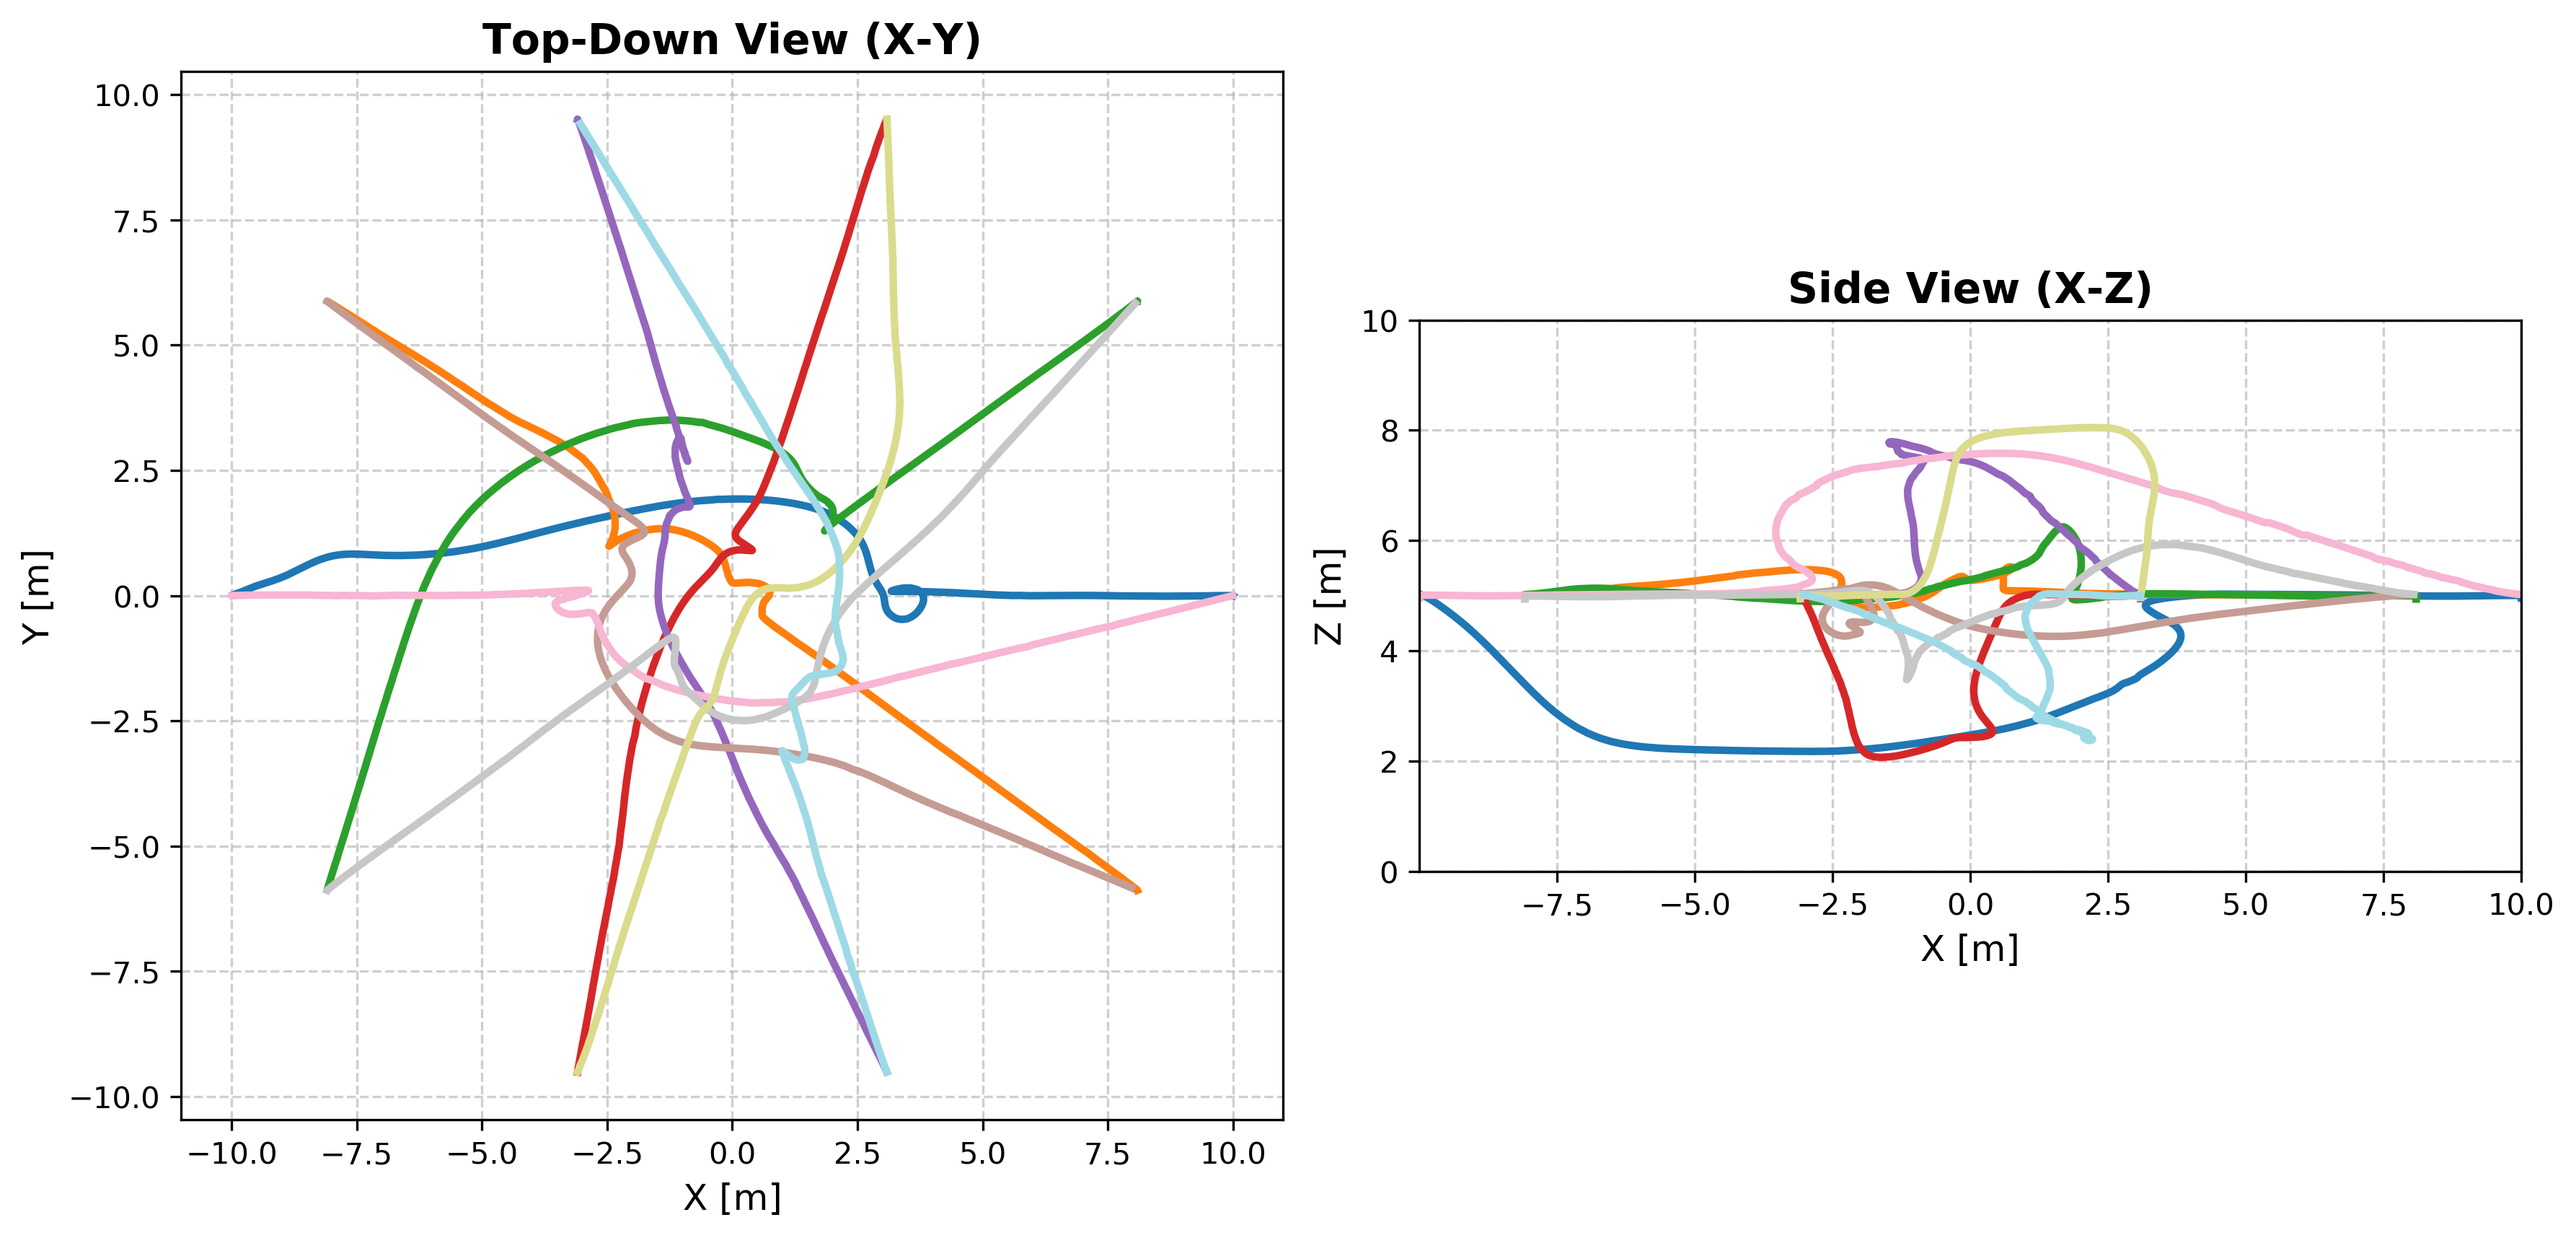
\includegraphics[width=0.48\textwidth, height=0.24\textwidth]{./fig/plots/n_10_circle_z_rule.png}
                \label{fig:n_10_circle_z_rule}
            }
            \par\medskip
            \subfloat[Trajectories of \ac{UAV}s using 3D \ac{RBL} on sphere, $N=10$] {
                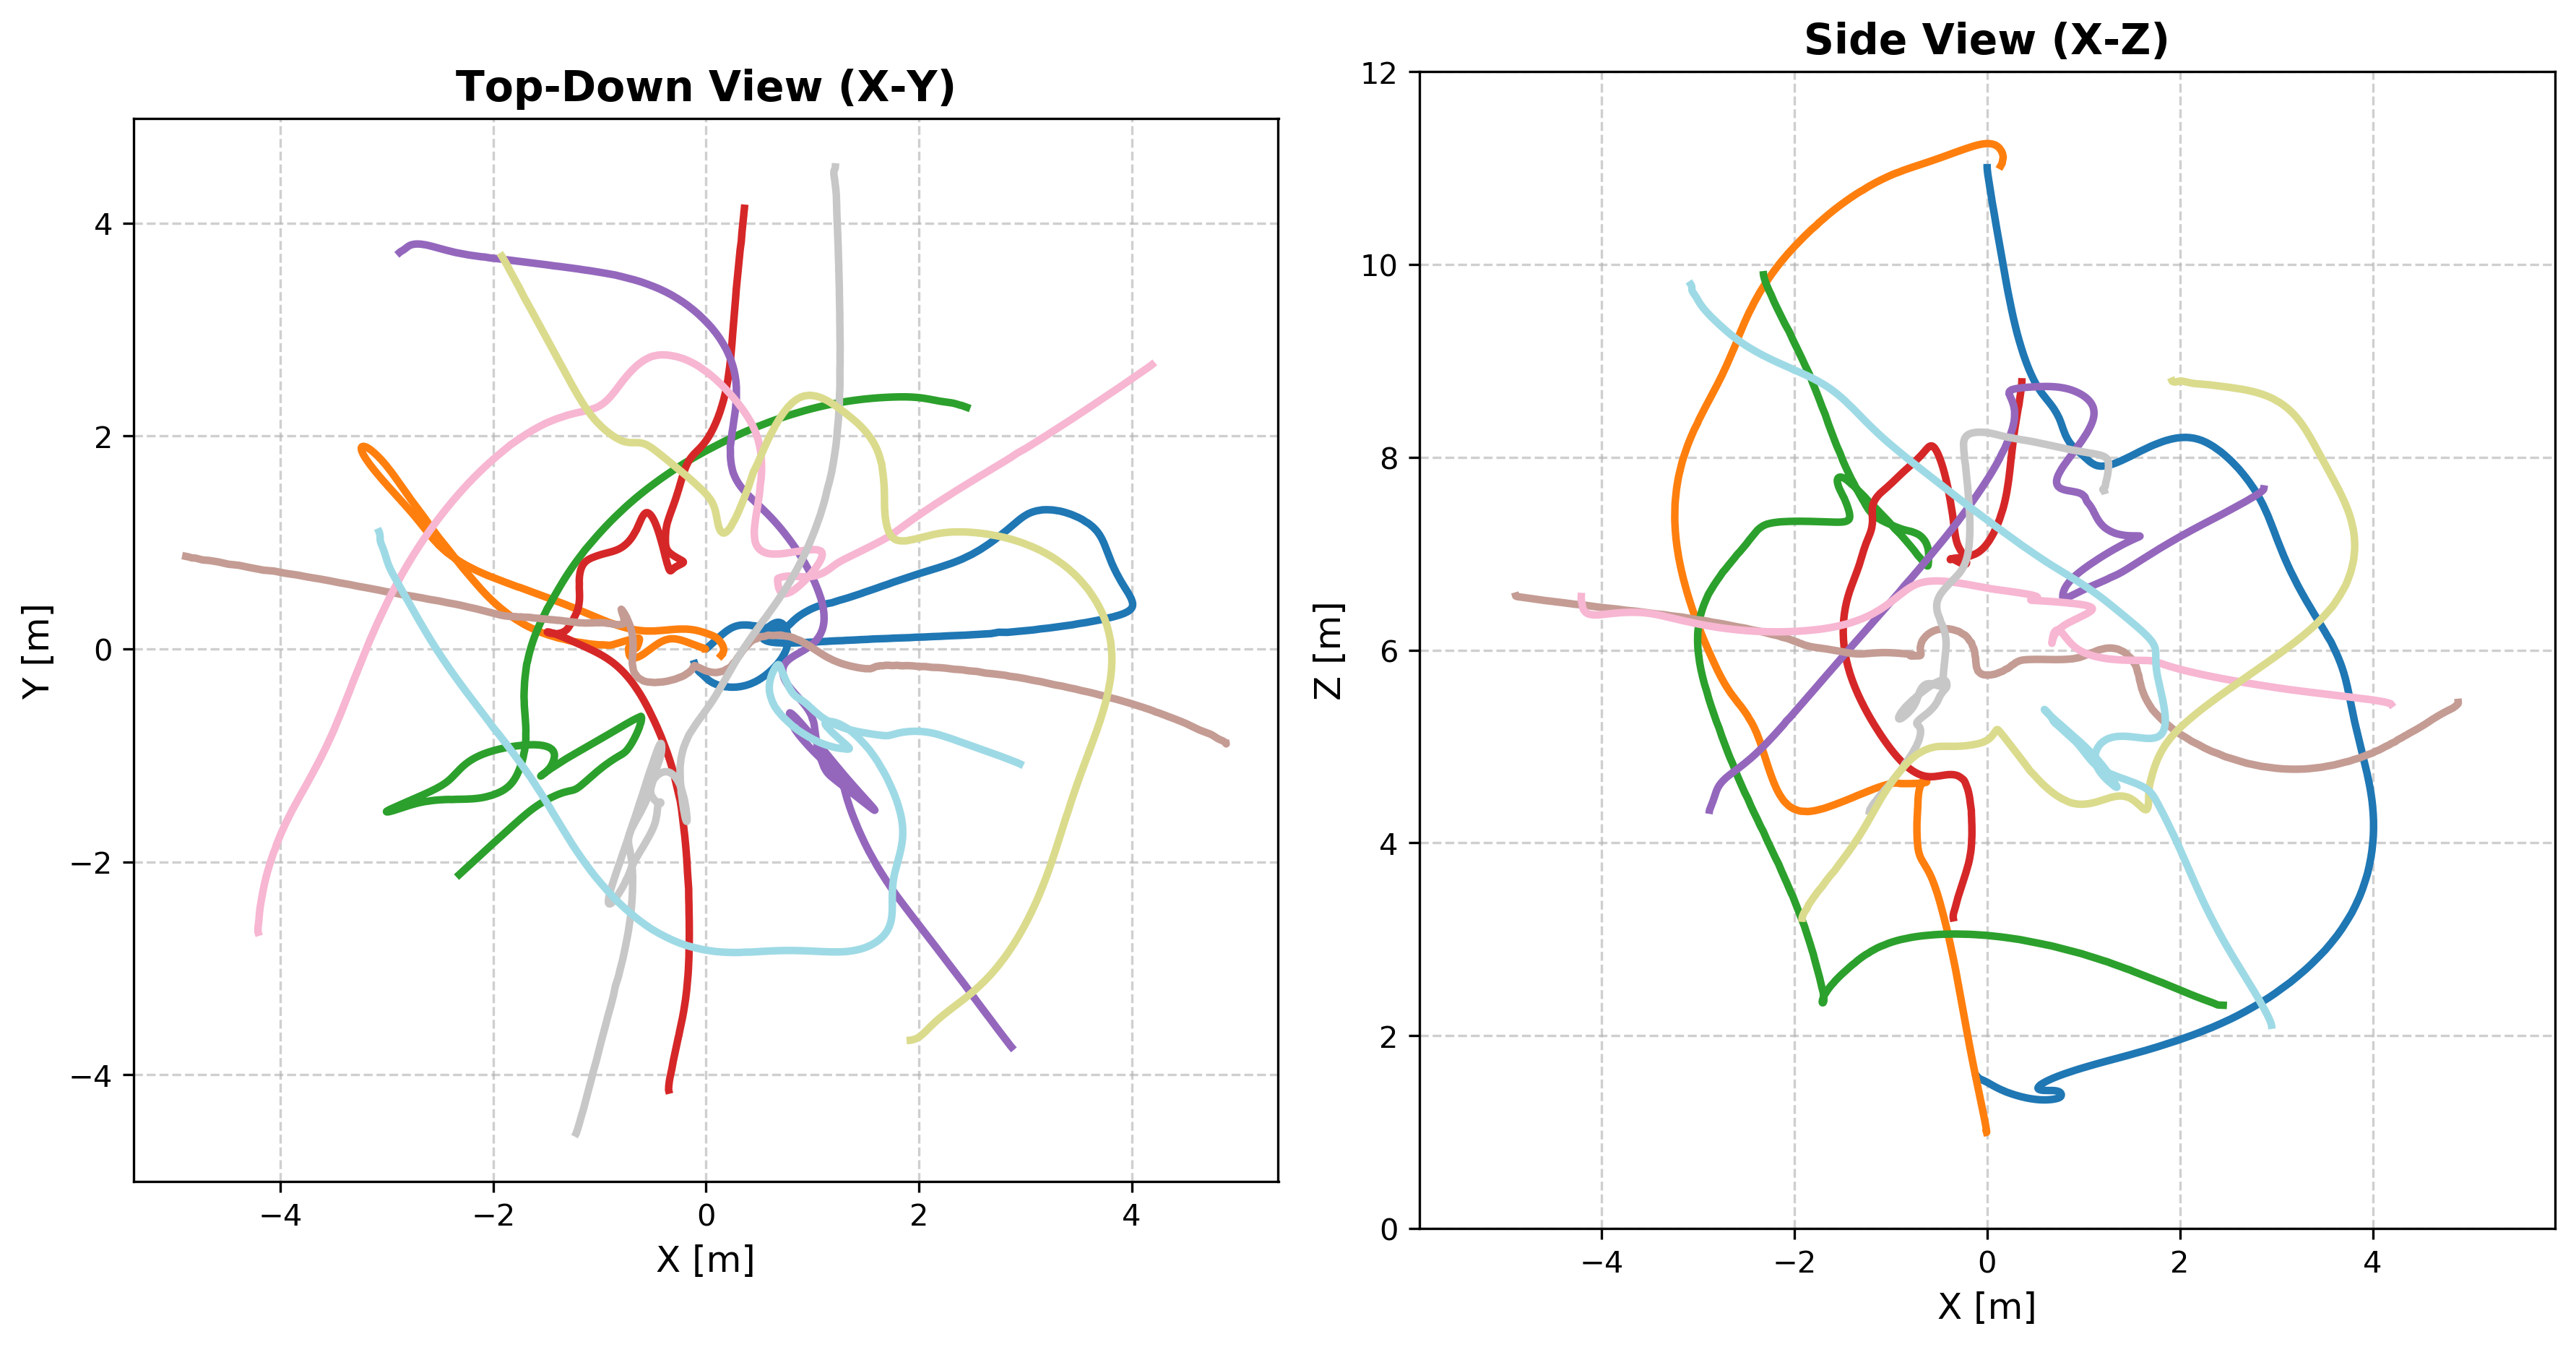
\includegraphics[width=0.48\textwidth, height=0.24\textwidth]{./fig/plots/n_10_sphere.png}
                \label{fig:n_10_sphere}
            }
            \caption{
                Visualization of UAV formations and algorithm behavior for $N=10$ (shown with top-down and side views). 
                (a) Trajectories in a 2D circular crossing. 
                (b) Trajectories in a 3D circular crossing. 
                (c) Effect of Z-axis clipping on the circular crossing. 
                (d) Effect of the Z-axis rule on the circular crossing. 
                (e) Trajectories in a 3D spherical crossing.
            }
            \label{fig:trajectories}
        \end{figure}


            
\section{Summary and Key Insights}
    Recap of modifications. Faced challenges and solutions applied
